\documentclass[11pt]{article}

\usepackage[margin=1in]{geometry}
\usepackage[T1]{fontenc}
\usepackage[utf8]{inputenc}
\usepackage{lmodern}
\usepackage{amsmath,amssymb,amsthm,bm,mathtools}
\usepackage{booktabs}
\usepackage{graphicx}
\usepackage{caption}
\usepackage{xcolor}
\usepackage{hyperref}
\usepackage{enumitem}
\usepackage{float}

\hypersetup{colorlinks=true, linkcolor=blue!60!black, citecolor=blue!60!black, urlcolor=blue!60!black}

\newtheorem{theorem}{Theorem}
\newtheorem{proposition}{Proposition}
\newtheorem{remark}{Remark}

\newcommand{\R}{\mathbb{R}}
\newcommand{\E}{\mathbb{E}}
\newcommand{\Var}{\operatorname{Var}}
\newcommand{\Cov}{\operatorname{Cov}}
\newcommand{\Normal}{\mathcal{N}}

\title{BP-Informed Diffusion Scores for Approximately Markovian Sequences\\
\large Calibrated grid BP, the message/model equivalence for single-Gaussian projections,\\
rank-one non-Markov corrections, hybrid residual learning, and reverse dynamics}
\author{Thesis project continuation --- second iteration}
\date{July 2026}

\begin{document}
\maketitle

\begin{abstract}
This report continues the study of belief-propagation (BP) computation of diffusion
scores for sequence data with (approximately) Markov structure. Building on the
previous note, we (i) audit and exactly reproduce the earlier package, identifying a
numerical boundary-collapse artifact in its grid-projected Gaussian BP that
contaminated all weak-noise results; (ii) prove that single-Gaussian moment-matched
(assumed-density) BP on any \emph{linear-transition} chain with Gaussian observation
factors is identical to exact Gaussian BP under the covariance-matched Gaussian model,
so that ``Gaussian message error'' and ``Gaussian model error'' coincide at this level;
(iii) calibrate grid BP against the exactly solvable Gaussian AR(1) case, finding
\emph{spectral} accuracy with an abrupt small-$t$ failure driven by likelihood
aliasing; (iv) quantify the corrected Gaussian-baseline error across heavy-tailed and
bimodal innovation families; (v) show that for Gaussian AR(1)-plus-global-latent priors
the non-Markov score correction is \emph{exactly rank one} at every diffusion time, and
that a neural network learning only this residual on top of a frozen Markov-BP score is
an order of magnitude more sample- and parameter-efficient than a direct score network;
and (vi) demonstrate in reverse-diffusion simulations that the Gaussian score
reproduces second-order statistics while completely washing out heavy-tailed
innovations, even though its trajectory-level effect is dynamically stable in the
$L^2$ sense. Throughout we separate exact statements from numerical approximations.
\end{abstract}

\tableofcontents
\newpage

%=====================================================================
\section{Setting and exact results}

\subsection{Model and forward convention}

Clean data $a_{1:n}\in\R^n$ follow a Markov chain prior
\begin{equation}
  p_0(a_{1:n}) = \mu(a_1)\prod_{i=2}^n K_i(a_i\mid a_{i-1}).
  \label{eq:markov-prior}
\end{equation}
The forward noising process is the coordinatewise Ornstein--Uhlenbeck
(variance-preserving) diffusion
\begin{equation}
  \mathrm dX_t = -X_t\,\mathrm dt + \sqrt2\,\mathrm dW_t,\qquad X_0 = a,
\end{equation}
whose transition kernel gives, at time $t$,
\begin{equation}
  x_i = \alpha_t a_i + \sqrt{\Delta_t}\,z_i,\qquad
  \alpha_t = e^{-t},\quad \Delta_t = 1-e^{-2t},\quad z_i\sim\Normal(0,1)\ \text{i.i.d.}
  \label{eq:ou}
\end{equation}
For unit-variance data, $\Var(x_i)=\alpha_t^2+\Delta_t=1$ at every $t$; all priors in
this report are normalized to unit marginal variance so that $p_T\to\Normal(0,I)$.
The sitewise likelihood is the exact Gaussian factor
$\ell_i(a_i;x_i)=\Normal(x_i;\alpha_t a_i,\Delta_t)$.

\subsection{Posterior chain, BP exactness, score identity}

Because the prior factorizes over adjacent pairs and the likelihood factorizes over
sites, the posterior is again a chain,
\begin{equation}
  p_t(a\mid x) \propto \mu(a_1)\prod_{i=2}^n K_i(a_i\mid a_{i-1})
  \prod_{i=1}^n \ell_i(a_i;x_i),
  \label{eq:posterior-chain}
\end{equation}
a tree-structured factor graph on which sum-product BP computes exact marginals
$b_i(a_i)=p_t(a_i\mid x)$ after one forward and one backward sweep (full derivations
in the previous report; they were checked line by line during the audit and are
correct). Combined with the denoising (Tweedie) identity for the OU kernel,
\begin{equation}
  \boxed{\;
  s_i(x,t) = \partial_{x_i}\log p_t(x)
  = -\frac{x_i - \alpha_t\, m_i(x,t)}{\Delta_t},
  \qquad m_i(x,t) = \E[a_i\mid x_{1:n}],\;}
  \label{eq:score-identity}
\end{equation}
this yields the exact theorem: \emph{for Markov-chain priors under coordinatewise OU
noising, BP computes the exact diffusion score}, provided messages are represented
exactly. The messages, however, are continuous functions; outside conjugate families
they admit no finite parametrization. Everything that follows concerns the
quantitative cost of representing them approximately, and what survives when the data
are only \emph{approximately} Markov.

\subsection{The master error identity}

If $\widehat m$ is any approximate posterior mean and
$\widehat s = -(x-\alpha_t\widehat m)/\Delta_t$, then for any reference pair
$(m_{\rm ref},s_{\rm ref})$ produced the same way,
\begin{equation}
  \boxed{\;\widehat s - s_{\rm ref} = \frac{\alpha_t}{\Delta_t}
  \bigl(\widehat m - m_{\rm ref}\bigr),\qquad
  \frac{\alpha_t}{\Delta_t}\sim\frac{1}{2t}\ \ (t\downarrow0).\;}
  \label{eq:error-identity}
\end{equation}
All score errors are amplified posterior-mean errors, with amplification diverging at
small noise. Every experiment in this package logs the numerical residual of
\eqref{eq:error-identity} (column \texttt{identity\_residual}); it is at machine
precision ($10^{-15}$--$10^{-12}$) throughout, as it must be, since it is algebra, not
approximation. (When the compared scores agree to machine precision the \emph{relative}
residual is $0/0$ and meaningless; the tables flag this case.)

Two further decompositions organize the study. Against an exact score,
\begin{equation}
  \widehat s - s_{\rm true}
  = \underbrace{(\widehat s - s_{\rm grid})}_{\text{message/model approx.}}
  + \underbrace{(s_{\rm grid} - s_{\rm true})}_{\text{grid discretization}},
\end{equation}
and for approximately Markov data,
\begin{equation}
  s_{\rm true} = s_{\rm Markov} + s_{\rm residual},
  \qquad
  s_{\rm hybrid,\theta} = s_{\rm BP,K_\varphi} + r_\theta .
  \label{eq:residual-decomp}
\end{equation}

%=====================================================================
\section{Audit of the previous package (Layer 1)}

The previous package was rerun under its documented configuration
(\texttt{--mode report --n-trials 12}, seed 11). All three CSV outputs reproduce
\emph{bit-for-bit up to machine precision} (largest deviation $2.1\times10^{-14}$,
attributable to numpy/BLAS version differences). The mathematical derivations match
the code. Two substantive findings change the interpretation of its results.

\paragraph{F1: boundary collapse of grid-projected Gaussian messages.}
The legacy \texttt{gaussian\_projected\_bp} evaluates each Gaussian message on the
grid, applies the exact grid update, and moment-matches the result. At weakly
informative times the outgoing message function is a near-flat ramp whose maximizer
lies \emph{outside} $[-A,A]$; moment-matching the truncated ramp yields a mean near the
grid boundary and a spuriously small variance, and the next update pushes it further
edge-ward (the backward integrand in $a$ peaks at $a'/\rho$, outside the grid) --- a
positive feedback loop. Diagnosed example (Gaussian prior, $t=1.8$): backward messages
collapse to $R_{\rm mean}\approx-7.7$, $R_{\rm var}\approx0.08$ on a $[-8,8]$ grid,
producing a posterior-mean error of $6.9$ at one site. This artifact---not Gaussian
closure---explains the anomalous large-$t$ rows of the previous package (posterior-mean
MSE $2.2\pm7.5$ at $t=1.3$ on the Laplace chain, and MSE up to $5.0$ in the
\emph{Gaussian} sanity check where projection should be exact).
Figure \ref{fig:artifact} quantifies the artifact against the corrected implementation:
it exceeds $6$ in posterior-mean sup-norm for $t\ge0.9$, precisely where the true
closure error is below $10^{-2}$.

\begin{figure}[H]
  \centering
  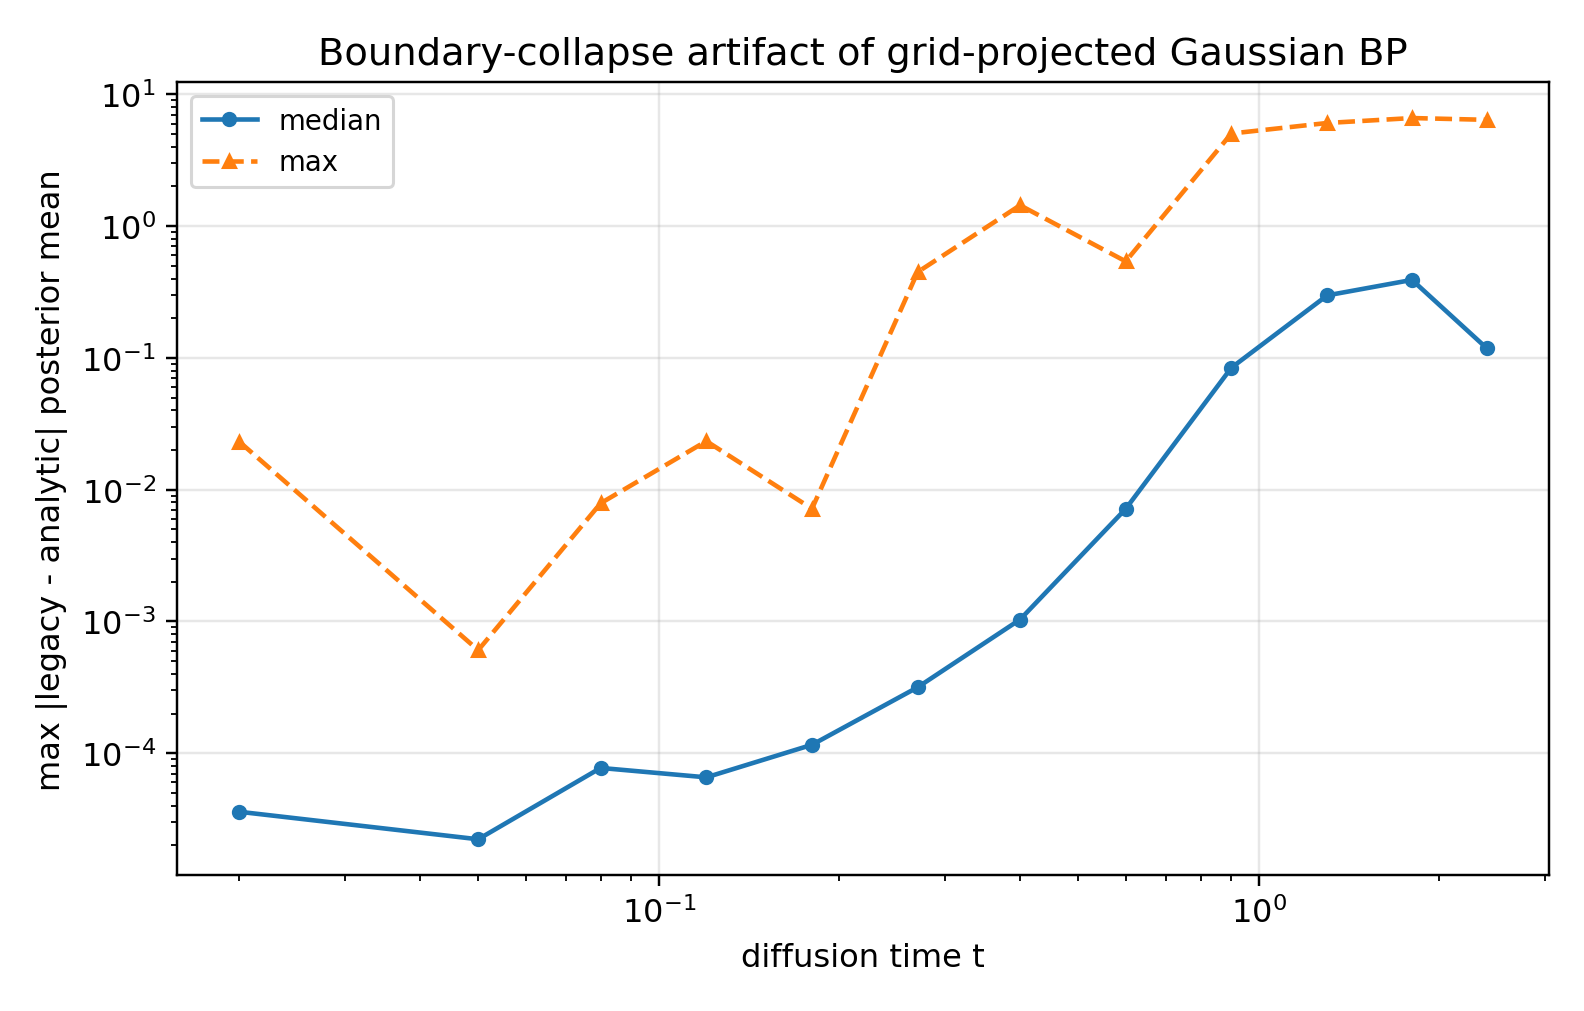
\includegraphics[width=0.72\textwidth]{../outputs/exp_02_laplace_gaussian_message_error/legacy_artifact_size.png}
  \caption{Audit finding F1. Sup-norm difference between the legacy grid-projected
  Gaussian BP posterior mean and the analytic information-form result on identical
  data (Laplace chain, $\rho=0.85$). The two implement the same projection map, so the
  difference is purely numerical. The large-$t$ explosion is the boundary-collapse
  artifact.}
  \label{fig:artifact}
\end{figure}

\paragraph{F2: message error $=$ model error for single-Gaussian projections.}
See Proposition \ref{prop:equivalence} below: what the previous package measured as
``Gaussian \emph{message} approximation error'' on the Laplace chain is mathematically
the error of the covariance-matched Gaussian \emph{model}. The numbers were right; the
interpretation needs sharpening. The distinction between message-level and model-level
approximation only becomes real for richer message families (mixtures, particles) or
nonlinear transitions.

Minor findings: grid sizes were compared on different random draws (fixed by common
random numbers keyed on $(\rho,t,\mathrm{trial})$); linear-domain likelihood rows can
underflow entirely for small $t$ (fixed by row-shifted log-likelihoods, exact because
per-site constants cancel); ad-hoc variance floors hid resolution failures (replaced by
an explicit resolution check). The corrected package returns, in addition, the exact
model evidence $\log p_t(x)$ from the BP normalization constants; it matches the
closed-form Gaussian marginal likelihood in the calibration case (unit test).

%=====================================================================
\section{Gaussian closure, and what a single Gaussian can ever measure}

In the Gaussian AR(1) case messages close in information form
$(\lambda, h)$: multiplication by the likelihood adds
$(\alpha_t^2/\Delta_t,\ \alpha_t x_i/\Delta_t)$, and the linear transition maps moments
$(m,v)\mapsto(\rho m,\ \rho^2 v + q)$. The corrected implementation
(\texttt{gaussian\_chain\_bp}) performs exactly these updates analytically; a flat
message is $\lambda=0$ exactly, so no truncated moment-matching ever occurs.

\begin{proposition}[Single-Gaussian ADF-BP $\equiv$ matched Gaussian model BP]
\label{prop:equivalence}
Let the clean chain have \emph{linear} transitions $a_i=\rho a_{i-1}+\varepsilon_i$
with $\E\varepsilon_i=0$, $\Var(\varepsilon_i)=q$, arbitrary innovation law, Gaussian
initial density, and Gaussian sitewise likelihoods \eqref{eq:ou}. Then assumed-density
BP that projects every message to a single Gaussian by moment matching produces
exactly the messages, beliefs, posterior means, and score of \emph{exact} BP under the
Gaussian AR(1) prior with the same $(\rho,q)$.
\end{proposition}

\begin{proof}
Forward pass: if the incoming message $L_i$ is Gaussian, the tilted product
$L_i\cdot\ell_i$ is a product of Gaussians, hence exactly Gaussian
$\Normal(\tilde m,\tilde v)$ --- projection is the identity here. The outgoing message
is the law of $\rho\xi+\varepsilon$ with $\xi\sim\Normal(\tilde m,\tilde v)$; whatever
the innovation law, its first two moments are $(\rho\tilde m,\ \rho^2\tilde v+q)$, so
the moment-matched Gaussian is $\Normal(\rho\tilde m,\rho^2\tilde v+q)$ --- identical
to the Gaussian-innovation update. Backward pass: the outgoing function is
$a\mapsto\E_\varepsilon[\tilde g(\rho a+\varepsilon)]=(\tilde g*\check p_\varepsilon)(\rho a)$
with $\tilde g=\Normal(\tilde m,\tilde v)$; the convolution has mean $\tilde m$ and
variance $\tilde v+q$ regardless of the innovation shape, so after the affine change of
variable the moment-matched message is $\Normal(\tilde m/\rho,(\tilde v+q)/\rho^2)$,
again the Gaussian-model update. By induction from the Gaussian initializations
($L_1=\mu$ Gaussian, $R_n$ flat), all message parameters coincide; beliefs are products
of Gaussians and coincide as well.
\end{proof}

\begin{remark}
The projection discards the innovation law beyond its variance \emph{at every step},
so nothing non-Gaussian ever enters. Consequently: (i) the honest implementation of
the single-Gaussian baseline is the analytic information-form filter (no grid);
(ii) measuring ``message error'' distinct from ``model error'' requires message
families that can carry non-Gaussian information (Gaussian mixtures being the natural
next step --- with mixture incoming messages the tilted products are mixtures and
multimodality survives the transition step); (iii) the proposition fails for
\emph{nonlinear} transitions, where the tilted forward moments genuinely depend on the
innovation shape. This is verified numerically: the legacy grid projection agrees with
the analytic filter to $5\times10^{-3}$ sup-norm at moderate $t$ on the Laplace chain
(unit test), the residual being grid quadrature error.
\end{remark}

%=====================================================================
\section{Layer 2: calibrating grid BP on the exactly solvable case}

Grid BP represents messages by values on $M$ equispaced points in $[-A,A]$ with
trapezoidal quadrature. Experiment 01 sweeps $M\in\{101,201,401,801\}$,
$A\in\{4,\dots,8\}$, $t\in[0.005, 2.4]$, $\rho\in\{0.2,0.5,0.8,0.95\}$ against the
exact Gaussian score, with identical random data across all grid configurations.

\begin{figure}[H]
  \centering
  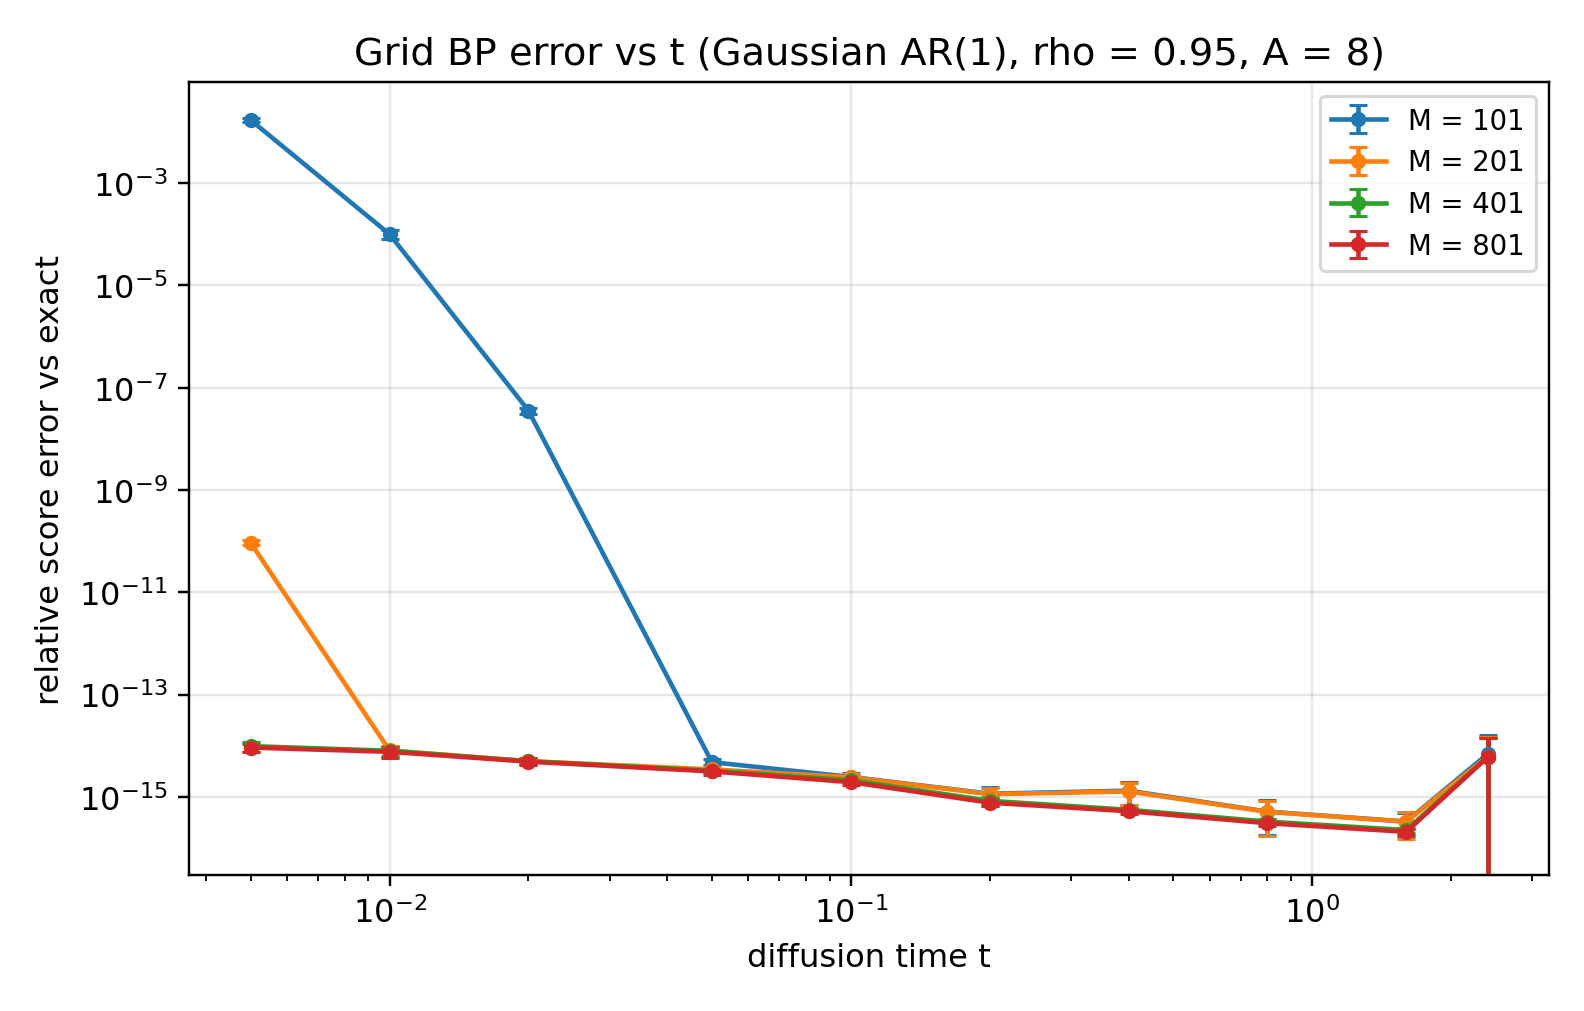
\includegraphics[width=0.72\textwidth]{../outputs/exp_01_grid_validation/grid_error_vs_t.png}
  \caption{Relative score error of grid BP vs the exact precision-matrix score
  ($\rho=0.95$, $A=8$). The error sits at the $10^{-15}$ floor except where the
  likelihood width $\sqrt{\Delta_t}/\alpha_t\approx\sqrt{2t}$ approaches the grid step:
  failure is abrupt, not gradual.}
  \label{fig:grid-t}
\end{figure}

\paragraph{Spectral accuracy.} The trapezoid rule on analytic, rapidly decaying
integrands converges exponentially in points-per-width (aliasing error
$\sim e^{-2\pi^2\sigma^2/\mathrm dx^2}$), not at the naive $O(\mathrm dx^2)$ rate.
Hence: at $M=101$, $A=8$ ($\mathrm dx=0.16$) the error is $10^{-15}$ down to $t=0.02$,
degrades to $10^{-4}$ at $t=0.01$, and fails ($1.7\times10^{-2}$) at $t=0.005$; at
$M=201$ it is at the floor for all tested $t$. Tail truncation is visible only at
$A=4$ (error $10^{-6}$--$10^{-4}$ depending on $\rho$; at $A=5$, $\le 7\times10^{-6}$
for Gaussian tails). See Figures \ref{fig:grid-MA}.

\begin{figure}[H]
  \centering
  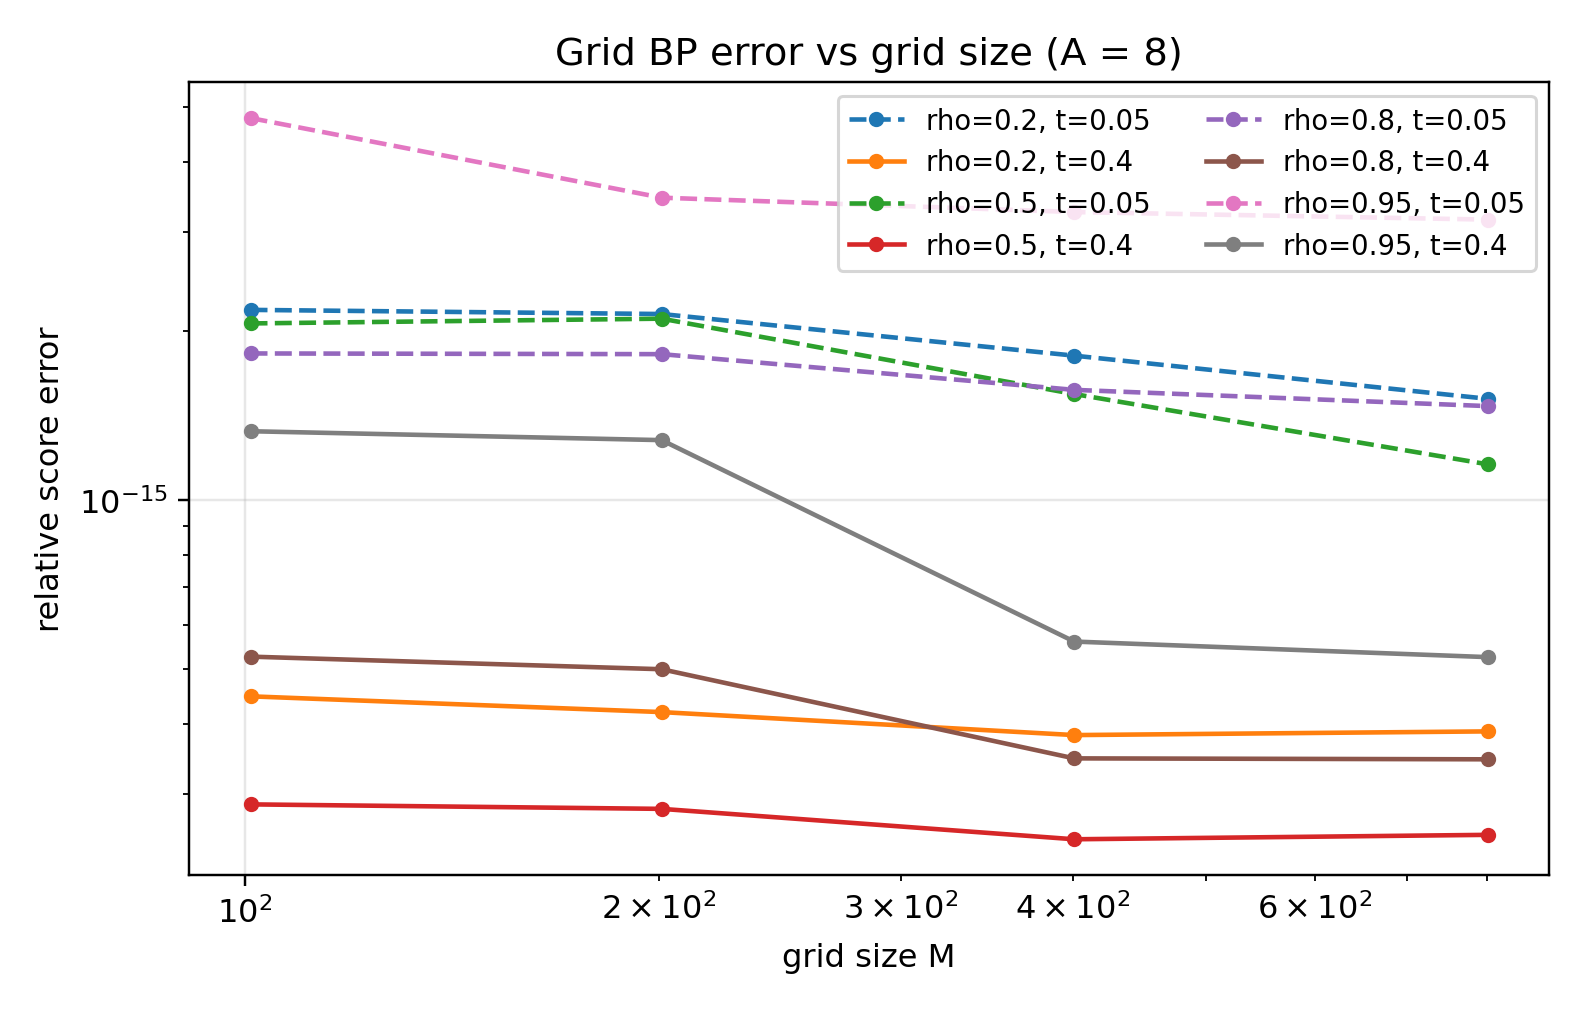
\includegraphics[width=0.49\textwidth]{../outputs/exp_01_grid_validation/grid_error_vs_M.png}
  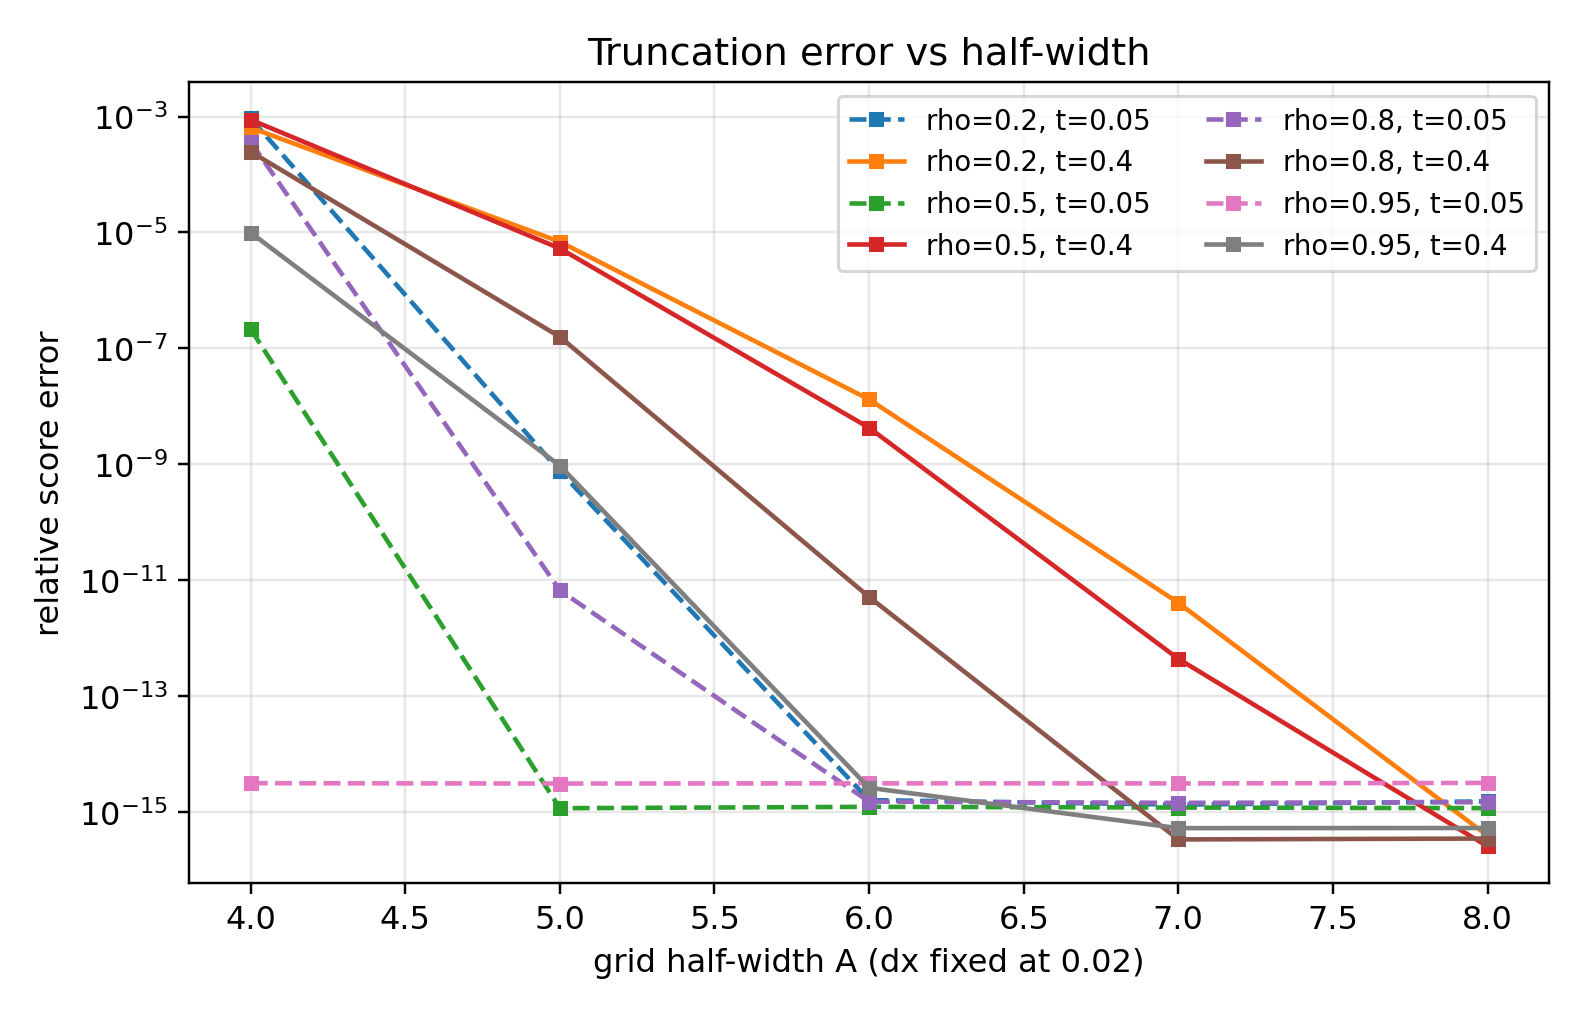
\includegraphics[width=0.49\textwidth]{../outputs/exp_01_grid_validation/grid_error_vs_A.png}
  \caption{Left: error vs $M$ at $A=8$. Right: error vs $A$ at fixed
  $\mathrm dx=0.02$ (truncation isolated).}
  \label{fig:grid-MA}
\end{figure}

\begin{figure}[H]
  \centering
  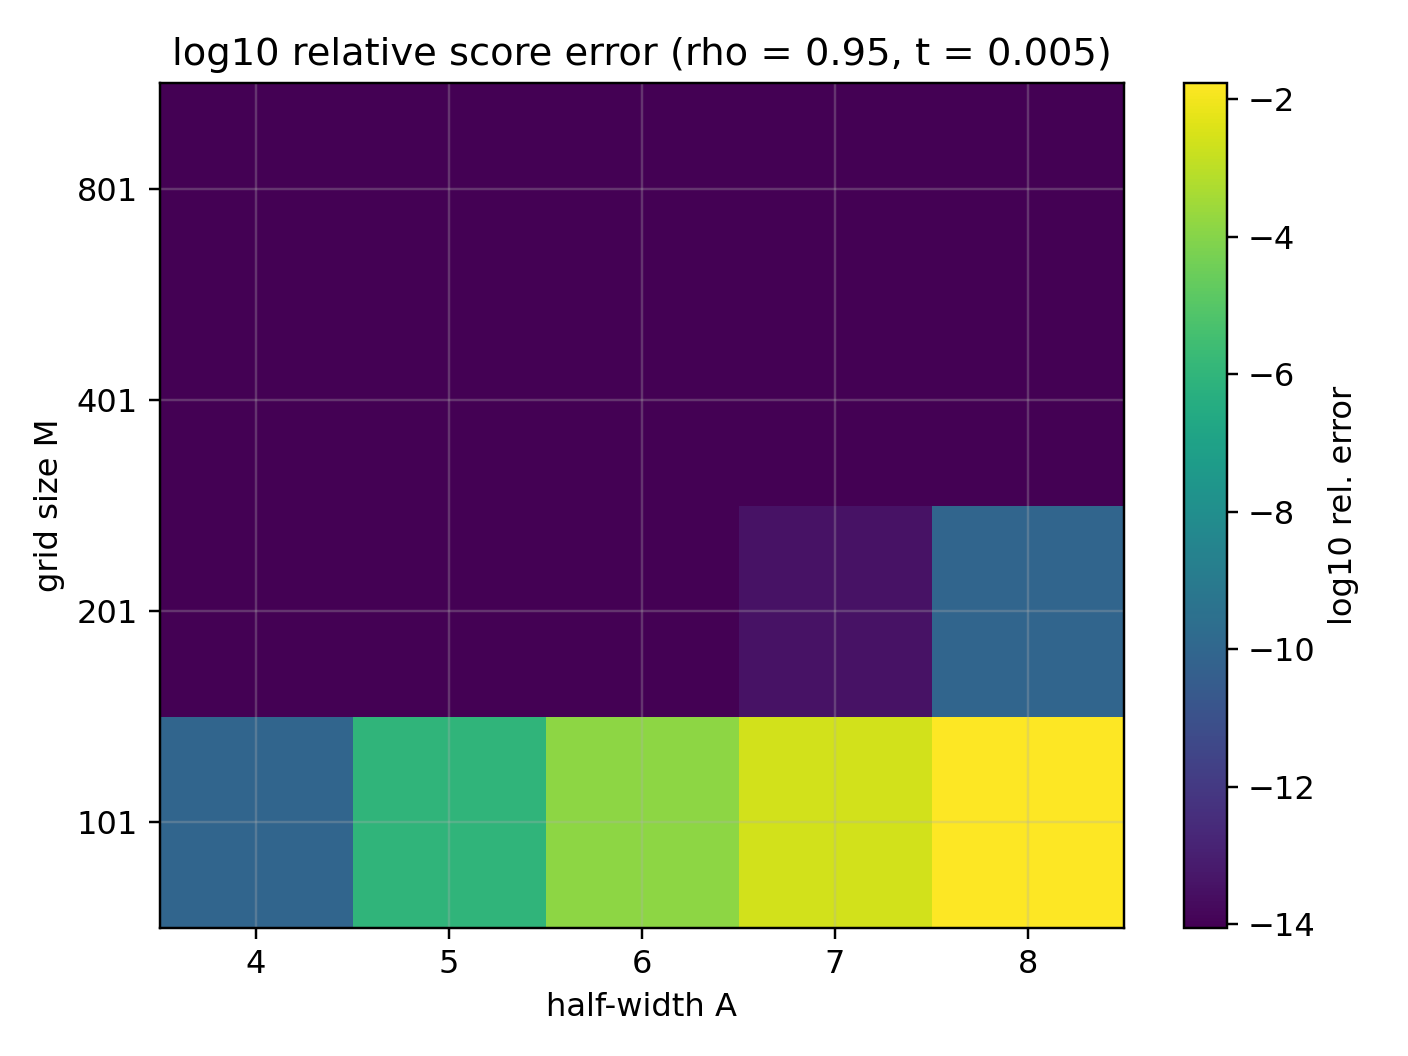
\includegraphics[width=0.49\textwidth]{../outputs/exp_01_grid_validation/grid_heatmap_t0.005.png}
  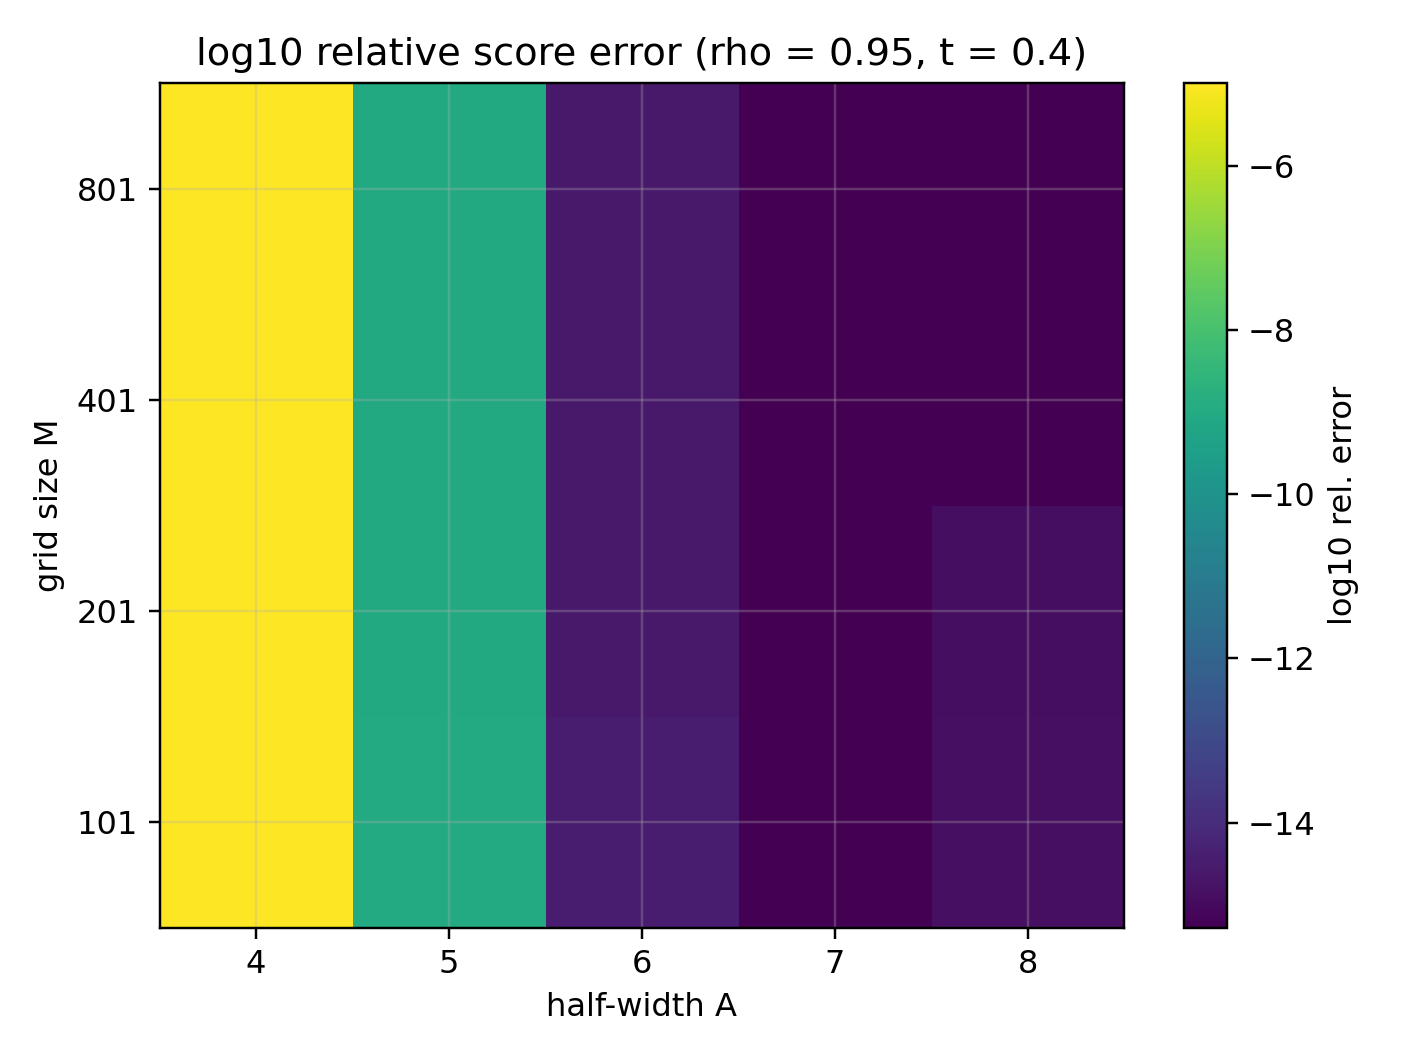
\includegraphics[width=0.49\textwidth]{../outputs/exp_01_grid_validation/grid_heatmap_t0.4.png}
  \caption{$(M,A)$ heatmaps of $\log_{10}$ relative score error at $\rho=0.95$;
  $t=0.005$ (left) shows the aliasing-driven failure region, $t=0.4$ (right) shows the
  truncation-only regime.}
  \label{fig:heatmap}
\end{figure}

\paragraph{Recommended defaults.} The Gaussian calibration alone would admit
$M=101$, $A=5$; because heavy-tailed innovations put more posterior mass in the tails,
we adopt $M=401$, $A=8$ as the working reference for all non-Gaussian experiments
(error floor in calibration, cost $O(nM^2)$ still trivial) and $M=801$ for convergence
checks. The binding small-$t$ constraint is $\sqrt{2t}\gtrsim 3\,\mathrm dx$, checked
automatically (\texttt{resolution\_ok}).

%=====================================================================
\section{Layer 3: the corrected Gaussian baseline on non-Gaussian chains}

\subsection{Laplace chain, per-trial analysis (exp.\ 02)}

On the Laplace chain ($\rho=0.85$, $n=40$, 60 trials per $t$, reference $M=801$,
$A=8$), the corrected baseline gives a clean monotone picture
(Figure \ref{fig:closure}): median relative score error $0.39$ at $t=0.02$, $0.17$ at
$t=0.08$, $3.5\times10^{-2}$ at $t=0.4$, $7.6\times10^{-5}$ at $t=2.4$. The failure
probability $P(\mathrm{err}>0.1)$ is $1$ for $t\le0.08$ and $0$ for $t\ge0.9$. The
grid self-convergence error ($M=401$ vs $801$) remains $10^{4}$--$10^{7}$ times
smaller than the closure error at every $t$: the reference is trustworthy where it is
used. The old package's large-$t$ anomalies are absent --- they were artifact F1.

\begin{figure}[H]
  \centering
  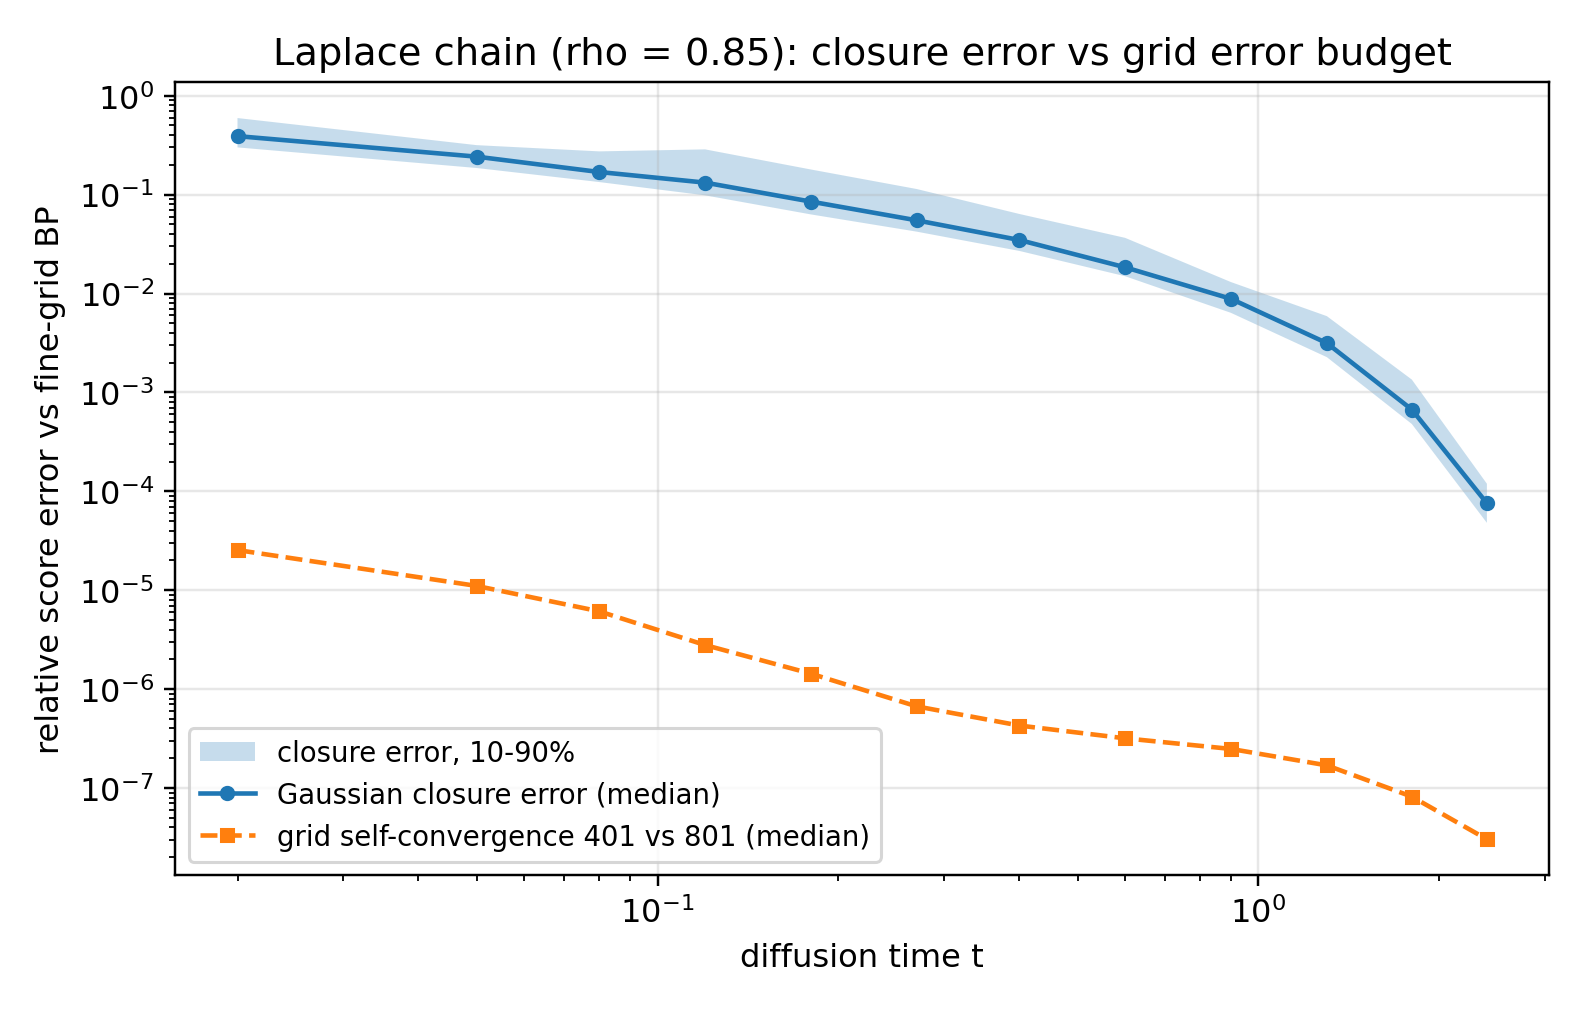
\includegraphics[width=0.72\textwidth]{../outputs/exp_02_laplace_gaussian_message_error/laplace_closure_vs_grid_budget.png}
  \caption{Gaussian closure error (median, 10--90\% band) vs the grid error budget on
  identical data. Laplace chain, $\rho=0.85$.}
  \label{fig:closure}
\end{figure}

\begin{figure}[H]
  \centering
  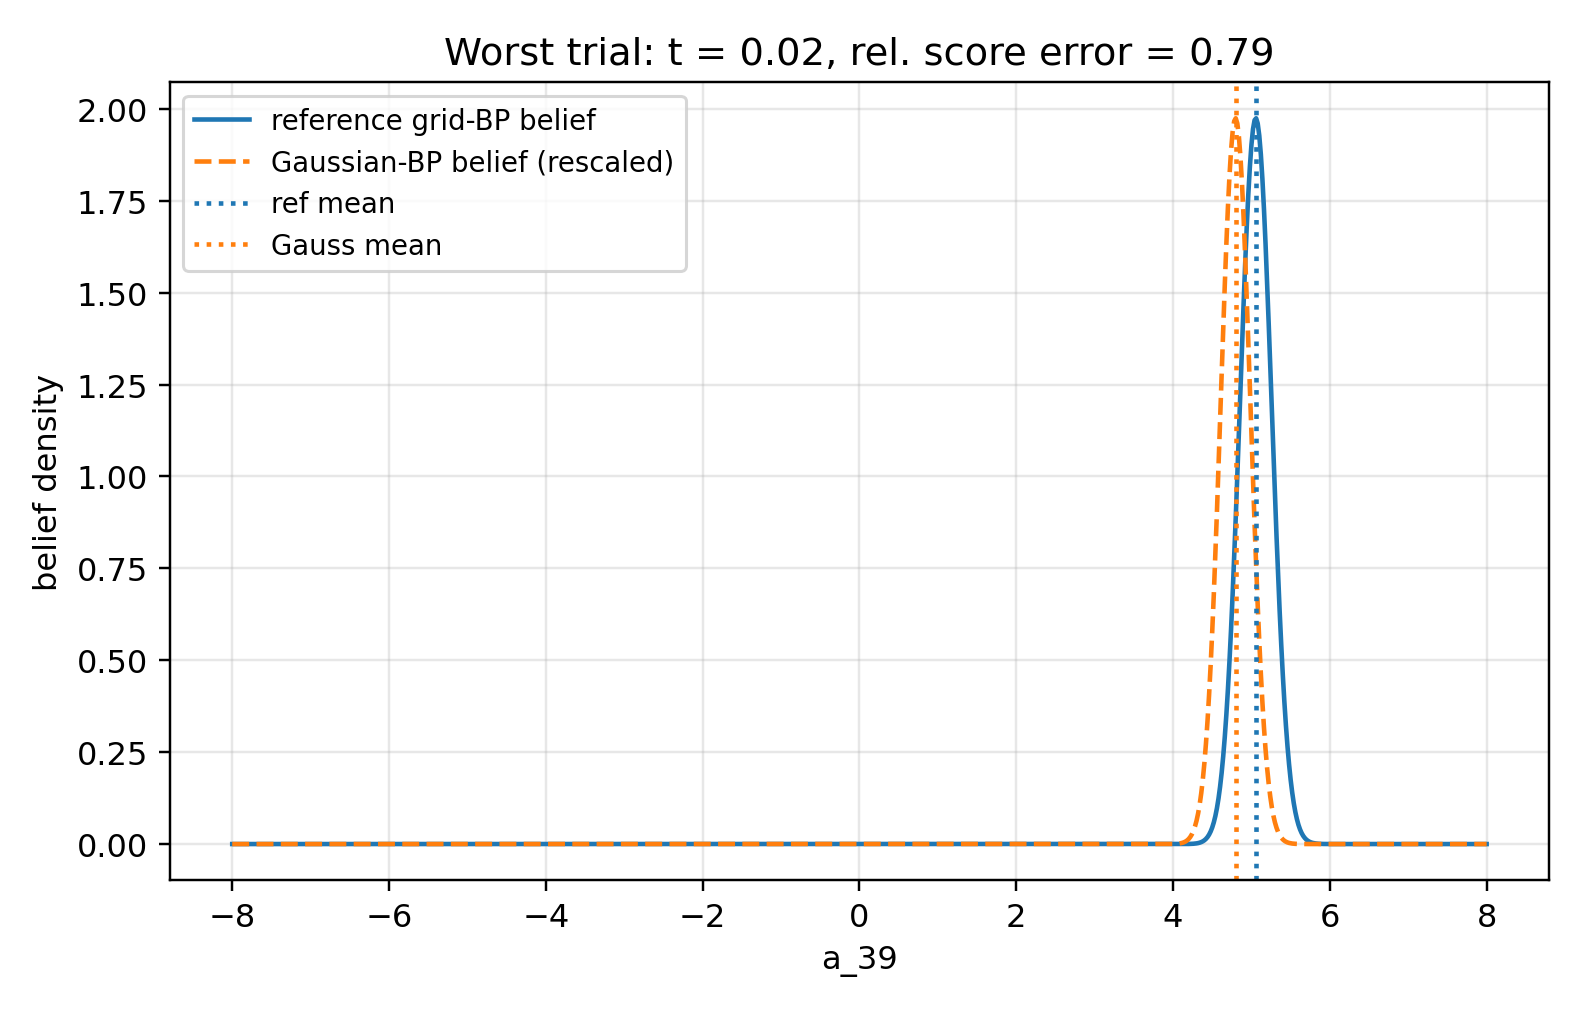
\includegraphics[width=0.6\textwidth]{../outputs/exp_02_laplace_gaussian_message_error/laplace_worst_case_belief.png}
  \caption{Worst trial across the sweep: the reference belief is sharply non-Gaussian
  and the single-Gaussian belief commits to a compromise; by
  \eqref{eq:error-identity} the mean shift is amplified by $\alpha_t/\Delta_t$.}
  \label{fig:worst}
\end{figure}

\subsection{Innovation sweep (exp.\ 03)}

Six families with \emph{identical} covariance $\rho^{|i-j|}$ and varying innovation
shape: Laplace (excess kurtosis $+3$), Student-$t$ with $\nu=5,8$ ($+6$, $+1.5$),
symmetric Gaussian mixtures with separation $\kappa=0.3,0.6,0.9$
($-0.18,-0.72,-1.62$; bimodal). Findings (Figure \ref{fig:sweep}, full table in
\texttt{outputs/exp\_03.../SUMMARY\_TABLE.md}):

\begin{itemize}[leftmargin=1.4em]
  \item \textbf{Noise level dominates}: every family's error decays to $\sim10^{-3}$
  or below by $t=2.4$; at high noise the Gaussian likelihood dominates the posterior
  and closure is nearly free. All meaningful error lives at $t\lesssim0.4$.
  \item \textbf{Both signs of non-Gaussianity hurt, bimodality hurts most}: at
  $t=0.05$, $\rho=0.5$: $\kappa=0.9$ mixture $0.94$, Laplace $0.52$, $t_{\nu=5}$
  $0.32$, $\kappa=0.3$ mixture $0.07$. Strongly bimodal innovations are the
  worst case at small $t$, matching the mechanism of Figure \ref{fig:worst}.
  \item \textbf{Stronger correlation helps, not hurts}: at fixed $t$ the error
  \emph{decreases} in $\rho$ (Laplace at $t=0.05$: $0.43$, $0.27$, $0.13$ for
  $\rho=0.5,0.85,0.95$). Informative neighbours act like extra Gaussian
  observations and Gaussianize the local tilted posterior. The naive intuition that
  message errors ``propagate farther'' at large $\rho$ is not what happens on chains.
\end{itemize}

\begin{figure}[H]
  \centering
  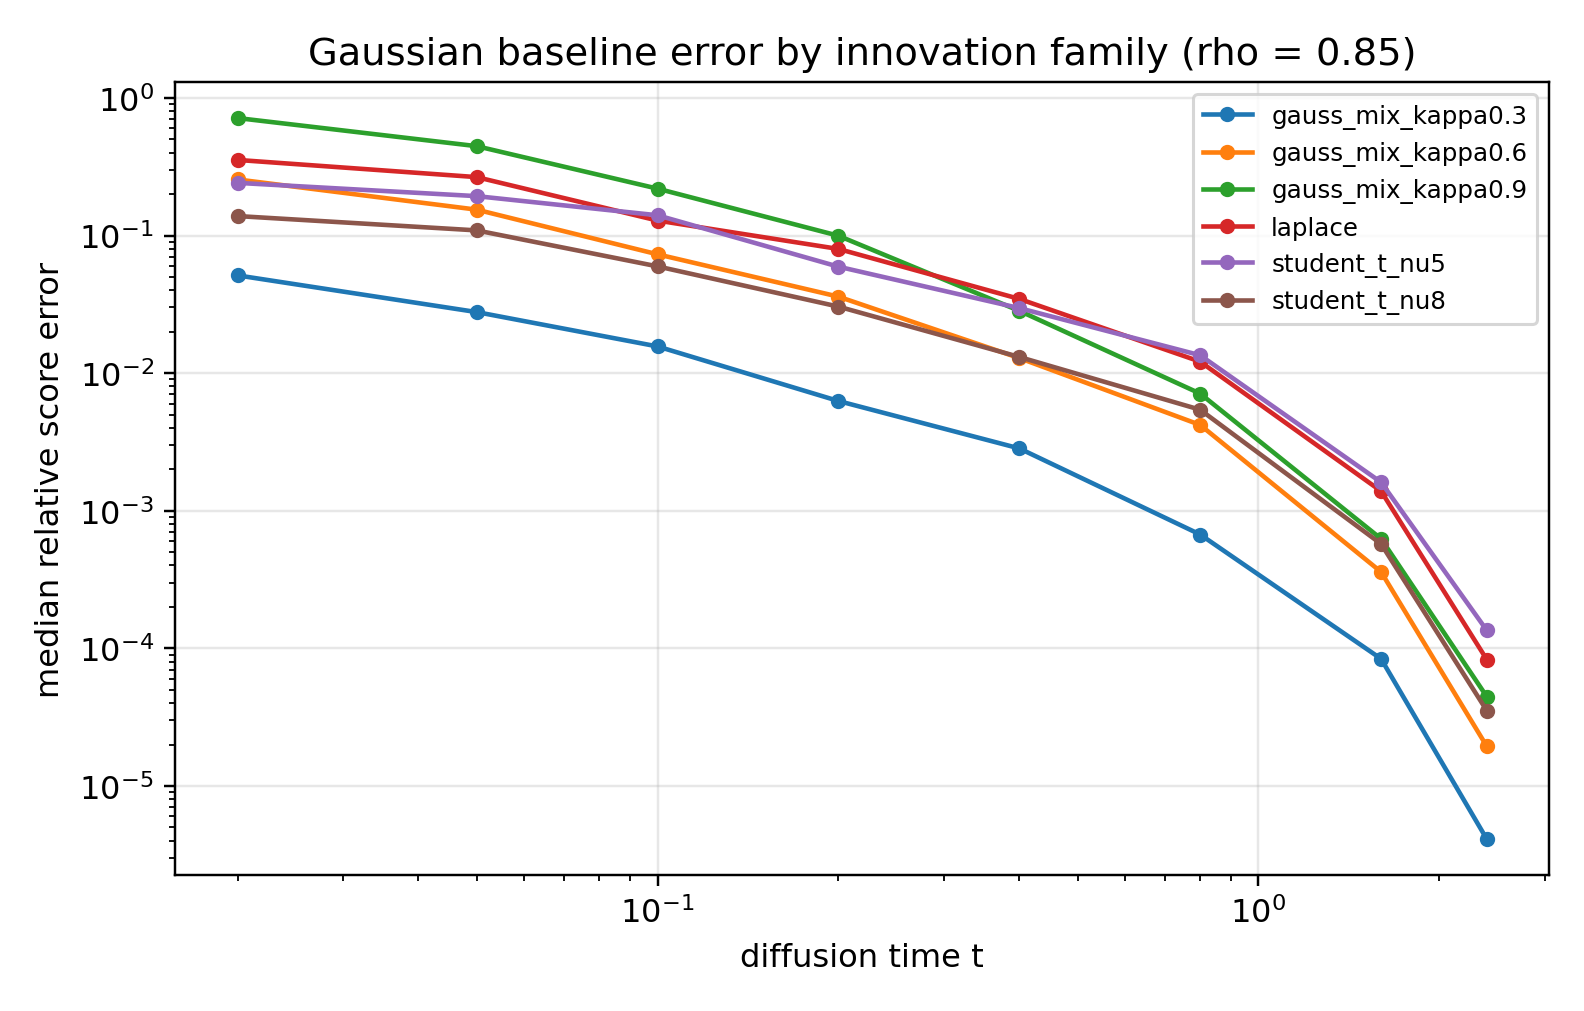
\includegraphics[width=0.49\textwidth]{../outputs/exp_03_nongaussian_innovation_sweep/sweep_error_vs_t.png}
  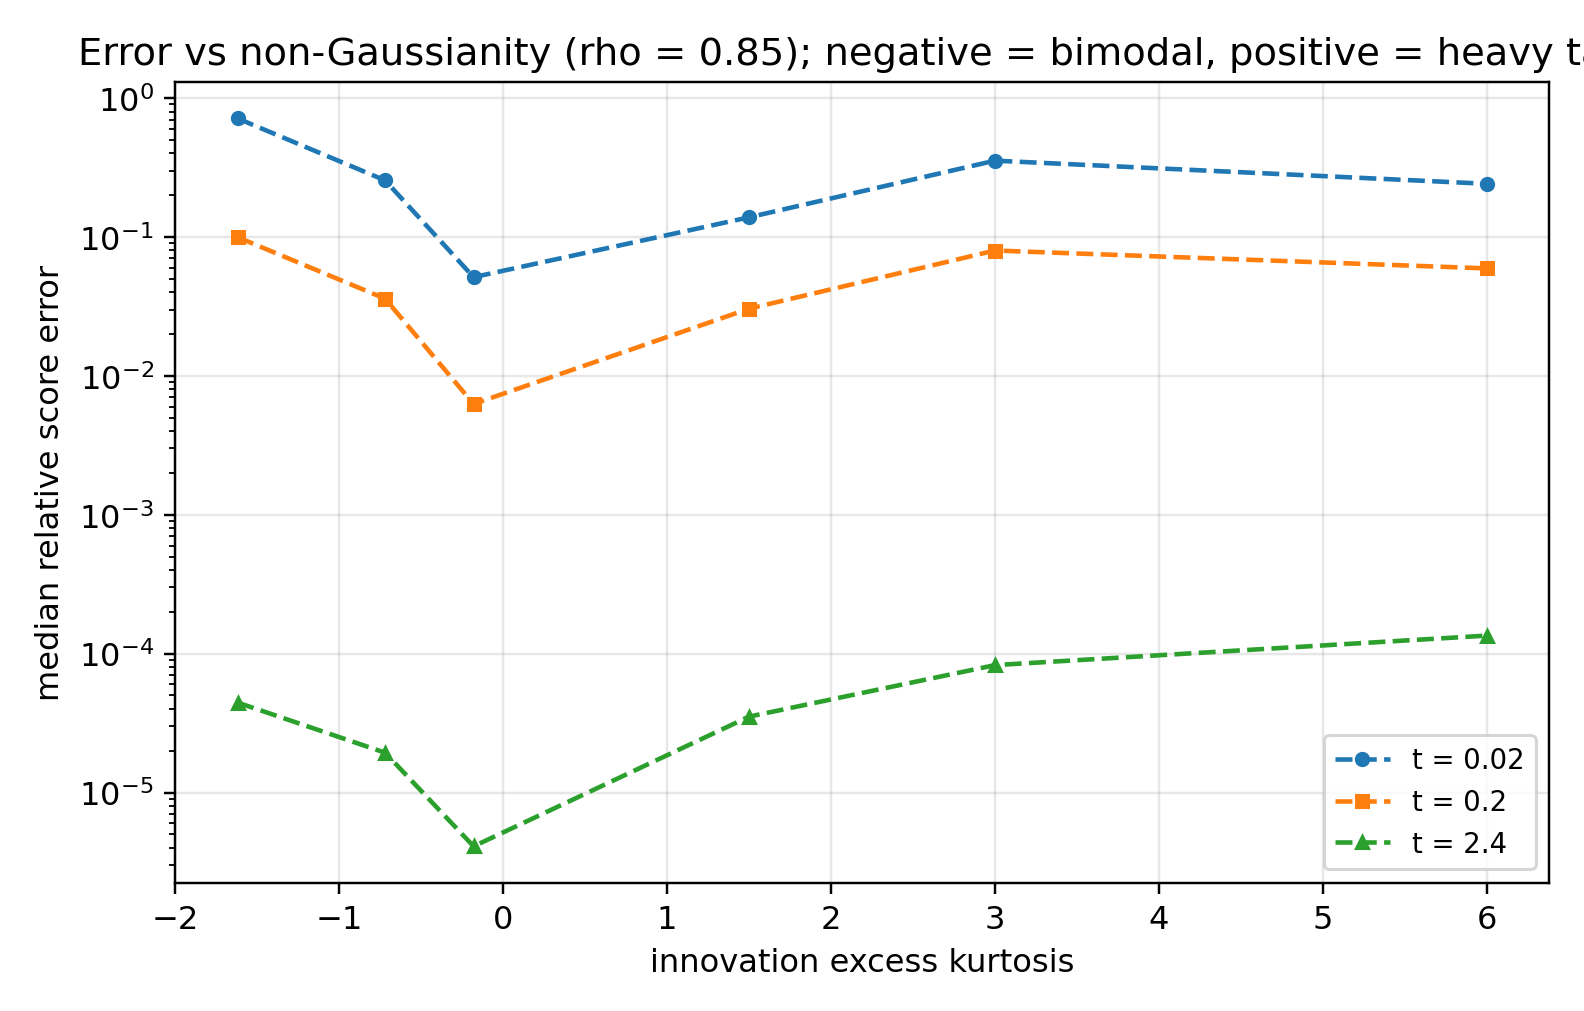
\includegraphics[width=0.49\textwidth]{../outputs/exp_03_nongaussian_innovation_sweep/sweep_error_vs_kurtosis.png}
  \caption{Left: median relative score error vs $t$ by family ($\rho=0.85$).
  Right: error vs innovation excess kurtosis (negative $=$ bimodal, positive $=$
  heavy-tailed) at three times.}
  \label{fig:sweep}
\end{figure}

By Proposition \ref{prop:equivalence} these numbers are simultaneously the
single-Gaussian \emph{message} error and the matched Gaussian \emph{model} error.
Separating the two requires mixture messages; this is the clearest next algorithmic
step and is left for the next iteration.

%=====================================================================
\section{Layer 4: approximate Markovianity}

Here the prior is \emph{not} a chain, but Gaussian, so every score is exact linear
algebra and the pure ``Markov approximation error'' is isolated with no grid and no
Monte Carlo in the operator analysis.

\subsection{Model A: AR(1) plus global latent --- the residual is rank one}

Let $a=(y+\beta g)/\sqrt{1+\beta^2}$ with $y$ a Gaussian AR(1)($\rho$) chain and
$g\sim\Normal(0,1)$ global, so
$\Sigma_0 = (\Sigma_y + \beta^2\mathbf1\mathbf1^\top)/(1+\beta^2)$.

\begin{proposition}[Rank-one non-Markov correction]\label{prop:woodbury}
Let $S_t=\alpha_t^2\Sigma_{\rm chain}+\Delta_t I$ be the noisy covariance of any chain
prior and let the true noisy covariance be $\Sigma_t = S_t + c\,\mathbf1\mathbf1^\top$
with $c=\alpha_t^2\beta^2/(1+\beta^2)$. Then by the Sherman--Morrison identity
\begin{equation}
  s_{\rm true}(x) - s_{\rm chain}(x)
  = \frac{c\,(\mathbf1^\top S_t^{-1}x)}{1 + c\,\mathbf1^\top S_t^{-1}\mathbf1}\;
    S_t^{-1}\mathbf1 ,
  \label{eq:rank-one}
\end{equation}
i.e.\ the non-Markov score correction is exactly rank one at every $t$: a fixed smooth
direction $S_t^{-1}\mathbf1$ with an $x$-linear scalar coefficient.
\end{proposition}

Numerically (exp.\ 04): the residual operator
$D_t=\Sigma_{{\rm chain},t}^{-1}-\Sigma_t^{-1}$ of the naive chain has
$\sigma_2/\sigma_1\sim10^{-12}$ (exact rank one), and chain-BP $+$ correction
\eqref{eq:rank-one} agrees with the exact score to $5\times10^{-14}$ --- this
\emph{is} augmented BP with the global latent integrated out in closed form. The
best-matched chain (Chow--Liu, adjacent pairwise marginals matched) has smaller
residual \emph{norm} (e.g.\ $0.066$ vs $0.086$ median relative residual at $\beta=1$,
$t=0.2$) but spreads it over many directions: structure and norm trade off. Residual
magnitudes are graceful in $\beta$: median relative score residual at $t=0.2$ of
$0.002/0.011/0.03/0.07$ for $\beta=0.1/0.25/0.5/1.0$ (Chow--Liu).

\begin{figure}[H]
  \centering
  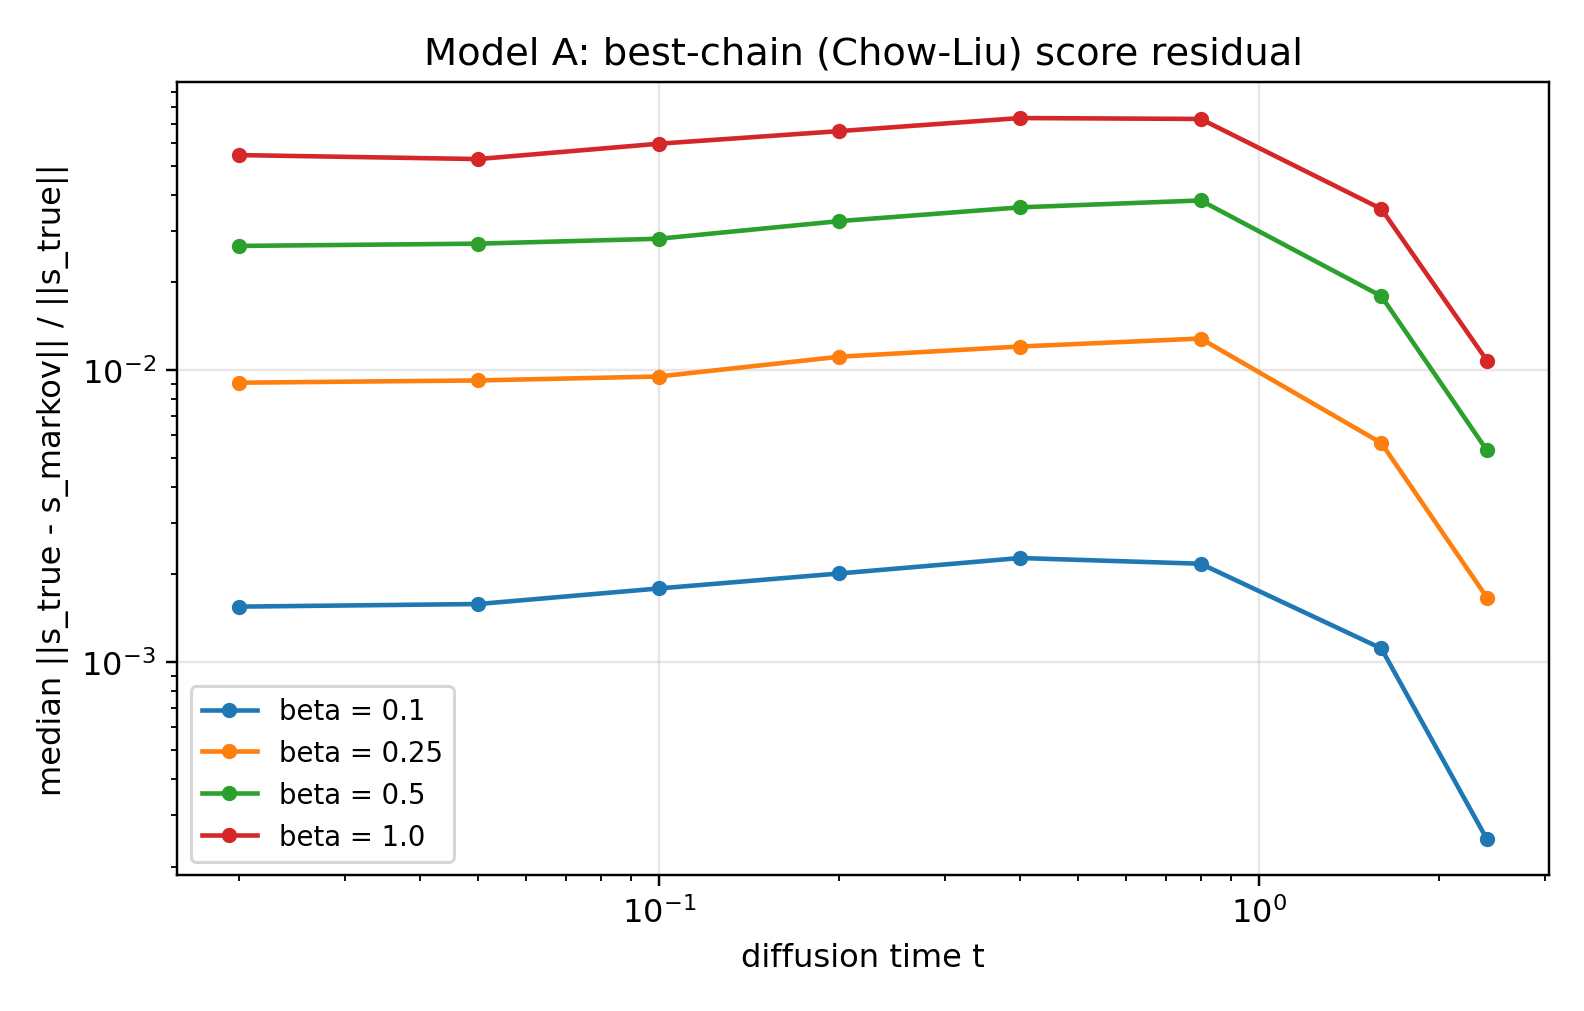
\includegraphics[width=0.49\textwidth]{../outputs/exp_04_approx_markovianity/modelA_residual_norm.png}
  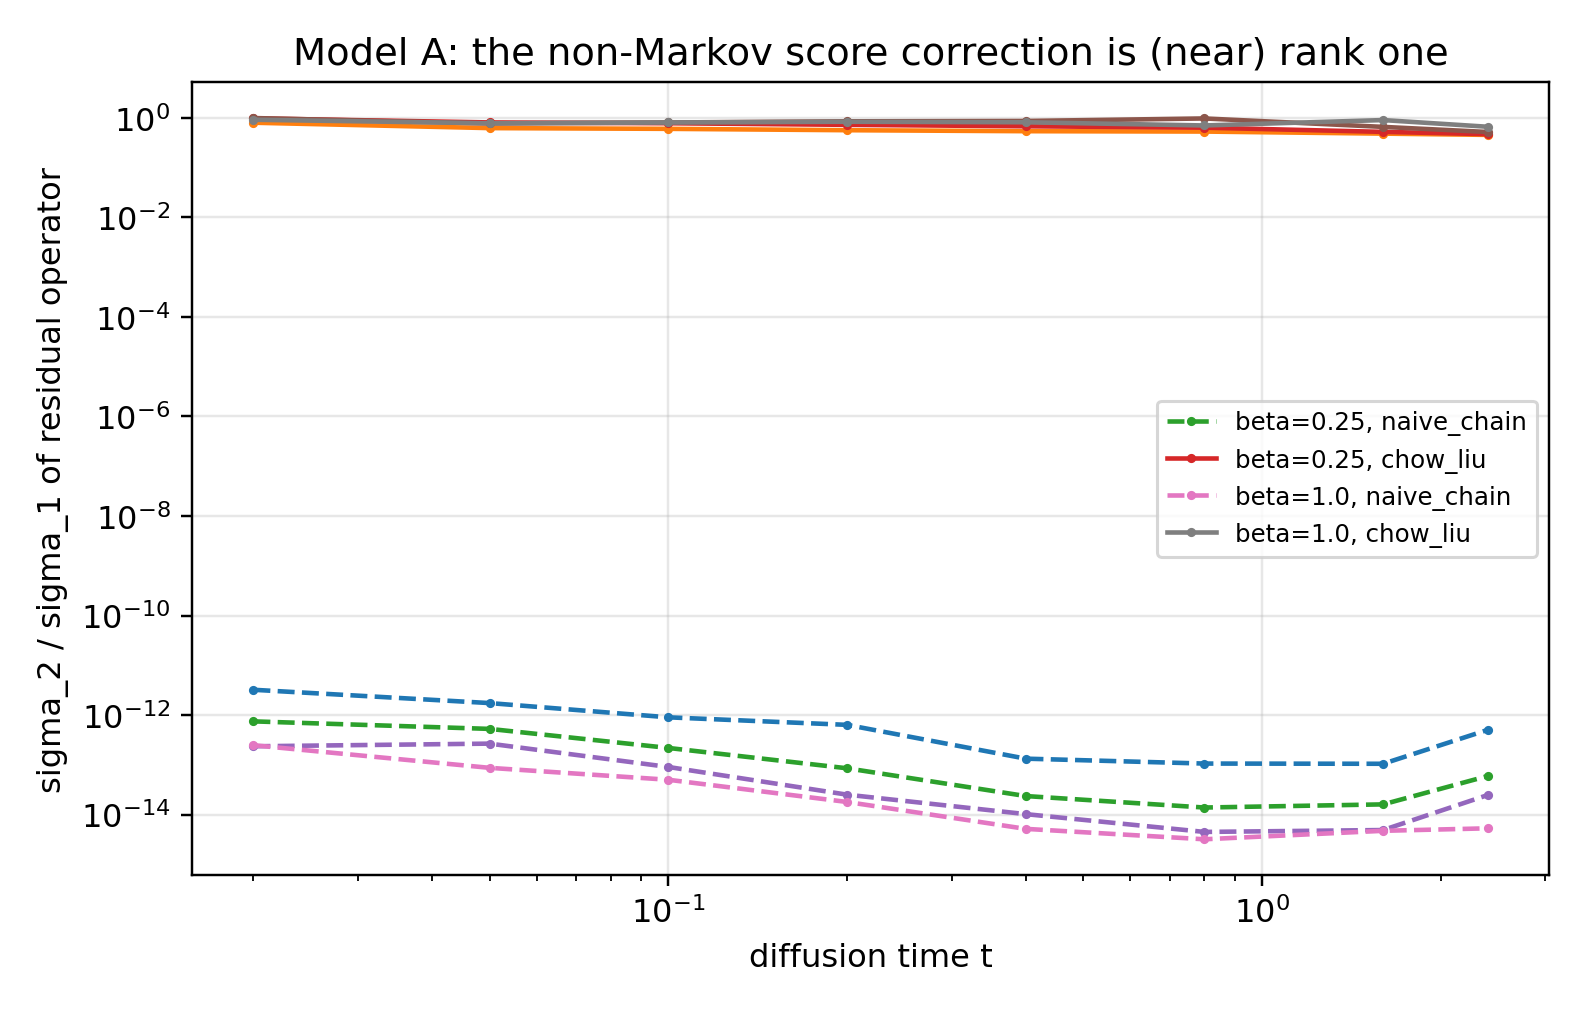
\includegraphics[width=0.49\textwidth]{../outputs/exp_04_approx_markovianity/modelA_rank_one_dominance.png}
  \caption{Model A. Left: relative score residual of the best chain approximation.
  Right: $\sigma_2/\sigma_1$ of the residual operator --- the naive chain's correction
  is exactly rank one (dashed, at numerical zero); Chow--Liu trades structure for
  norm.}
  \label{fig:modelA}
\end{figure}

\subsection{Model B: weak long-range precision coupling}

With $Q=Q_{\rm AR1}+\gamma Q_{\rm long}$ (exponentially decaying long-range couplings,
diagonally compensated, covariance renormalized to unit diagonal), the Chow--Liu chain
residual grows like $0.084/0.13/0.17/0.23$ (median, $t=0.2$) for
$\gamma=0.05/0.1/0.2/0.4$, with effective rank $\approx30$: a genuinely
high-rank correction. Low-rank latent structure (Model A) is the favourable regime for
Markov-plus-residual decompositions; generic long-range couplings are not, although
the residual \emph{norm} remains modest for weak $\gamma$.

\begin{figure}[H]
  \centering
  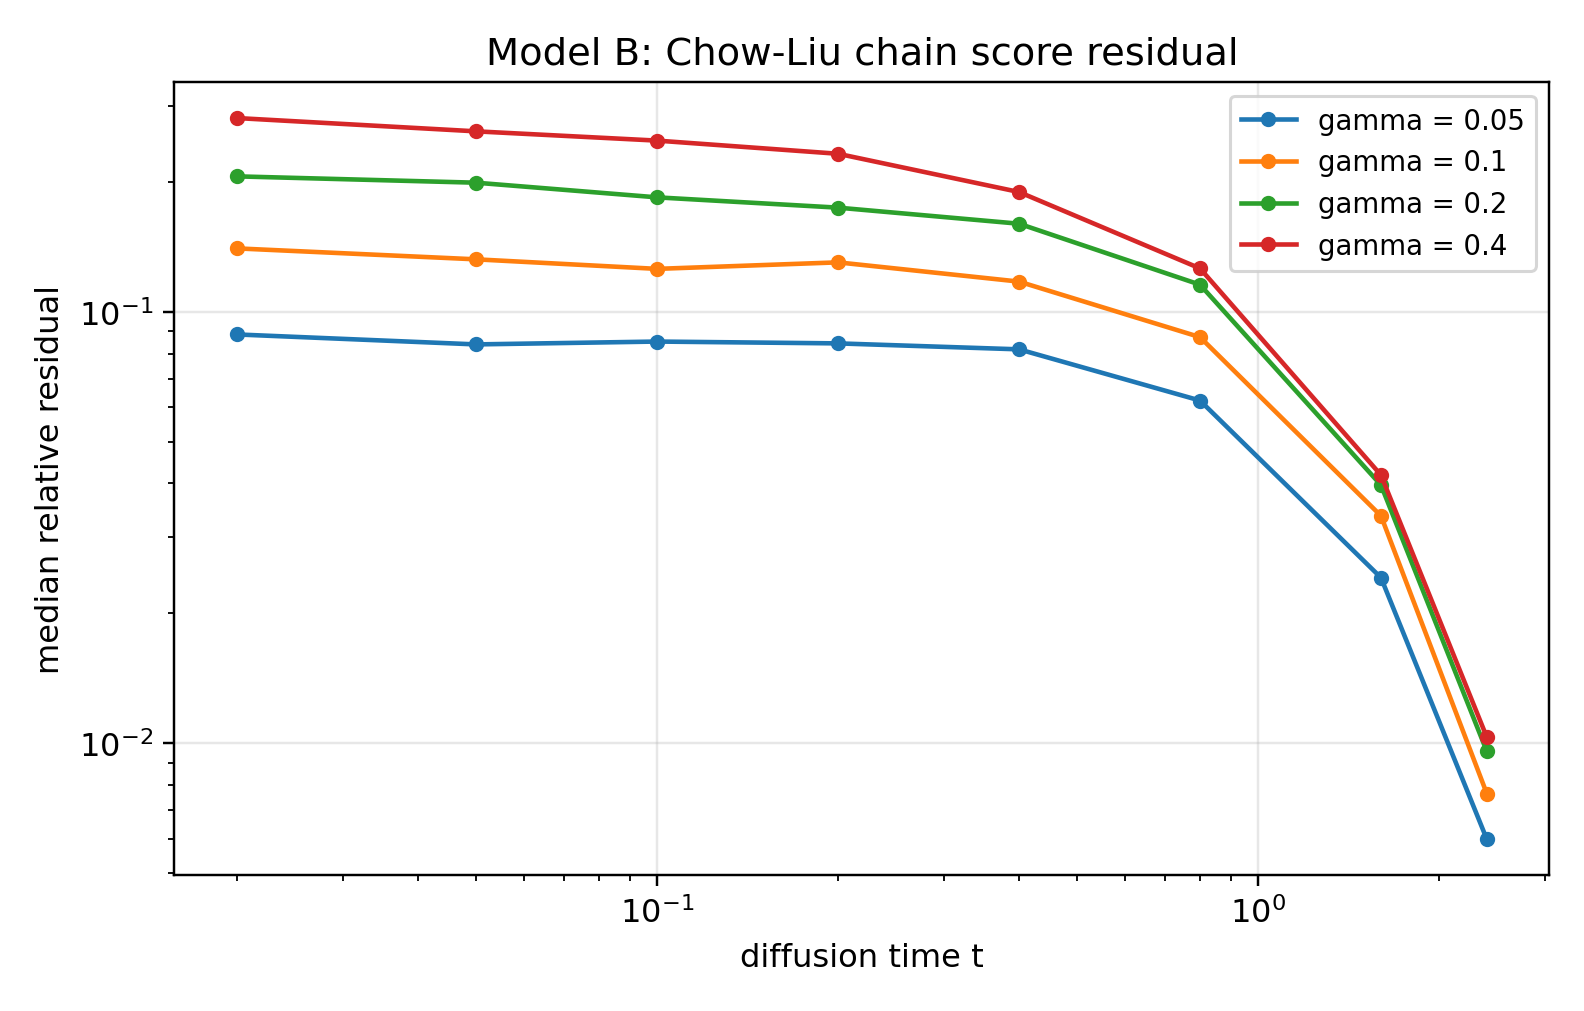
\includegraphics[width=0.49\textwidth]{../outputs/exp_04_approx_markovianity/modelB_residual_norm.png}
  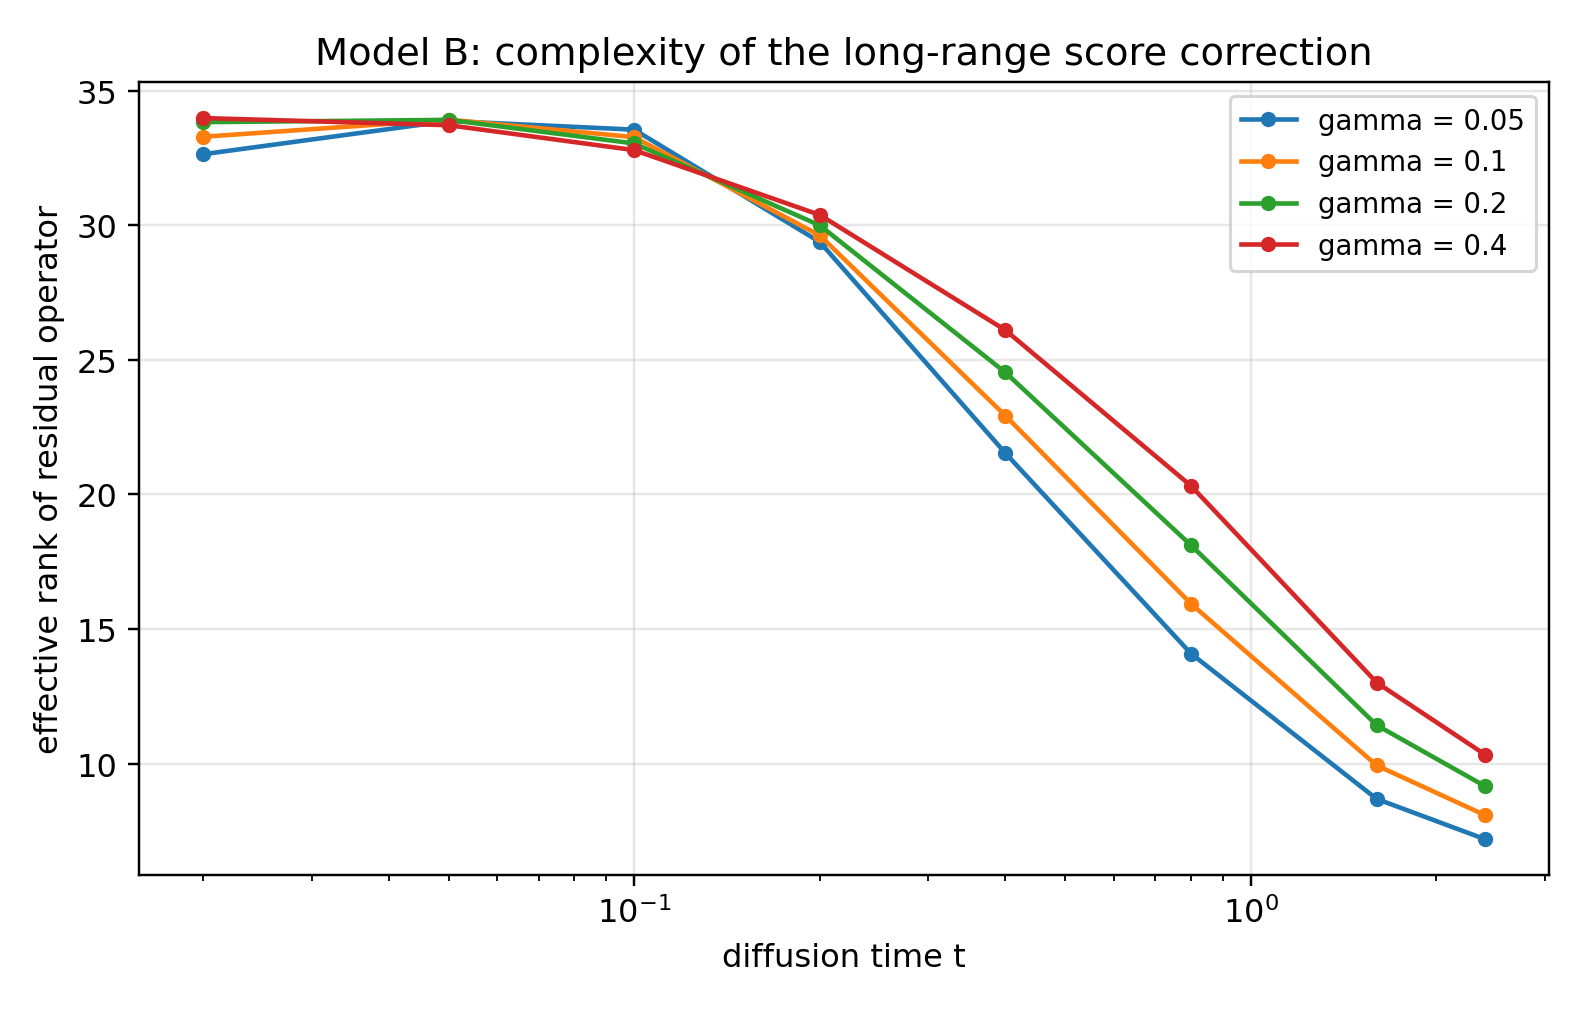
\includegraphics[width=0.49\textwidth]{../outputs/exp_04_approx_markovianity/modelB_effective_rank.png}
  \caption{Model B: residual norm (left) and effective rank of the residual operator
  (right).}
  \label{fig:modelB}
\end{figure}

\subsection{Hybrid learning: BP baseline plus neural residual}

On Model A ($\beta=0.5$, $\rho=0.8$, $n=40$), supervised regression on exact-score
targets, times log-uniform in $[0.02,3]$: a direct MLP $s_\theta(x,t)$ versus the
frozen Chow--Liu Markov-BP score plus an identical-architecture MLP learning only the
residual \eqref{eq:residual-decomp}. Test relative score error on 2048 held-out
samples:

\begin{center}
\begin{tabular}{lrrrr}
\toprule
$N_{\rm train}$ & 64 & 256 & 1024 & 4096\\
\midrule
direct MLP & 0.88 & 0.75 & 0.29 & 0.20\\
hybrid (BP $+$ residual MLP) & \textbf{0.23} & \textbf{0.060} & \textbf{0.015} & \textbf{0.014}\\
Markov BP alone (no learning) & \multicolumn{4}{c}{0.031}\\
\bottomrule
\end{tabular}
\end{center}

The hybrid improves on the free Markov baseline from 256 samples on and is
$\sim$20$\times$ better than the direct network at every size; the direct network does
not reach the \emph{no-learning} baseline even at 4096 samples. Parameter efficiency
is equally lopsided: a width-16 residual net (1.7k parameters, error $0.017$)
outperforms a width-256 direct net (87k parameters, error $0.33$).

\begin{figure}[H]
  \centering
  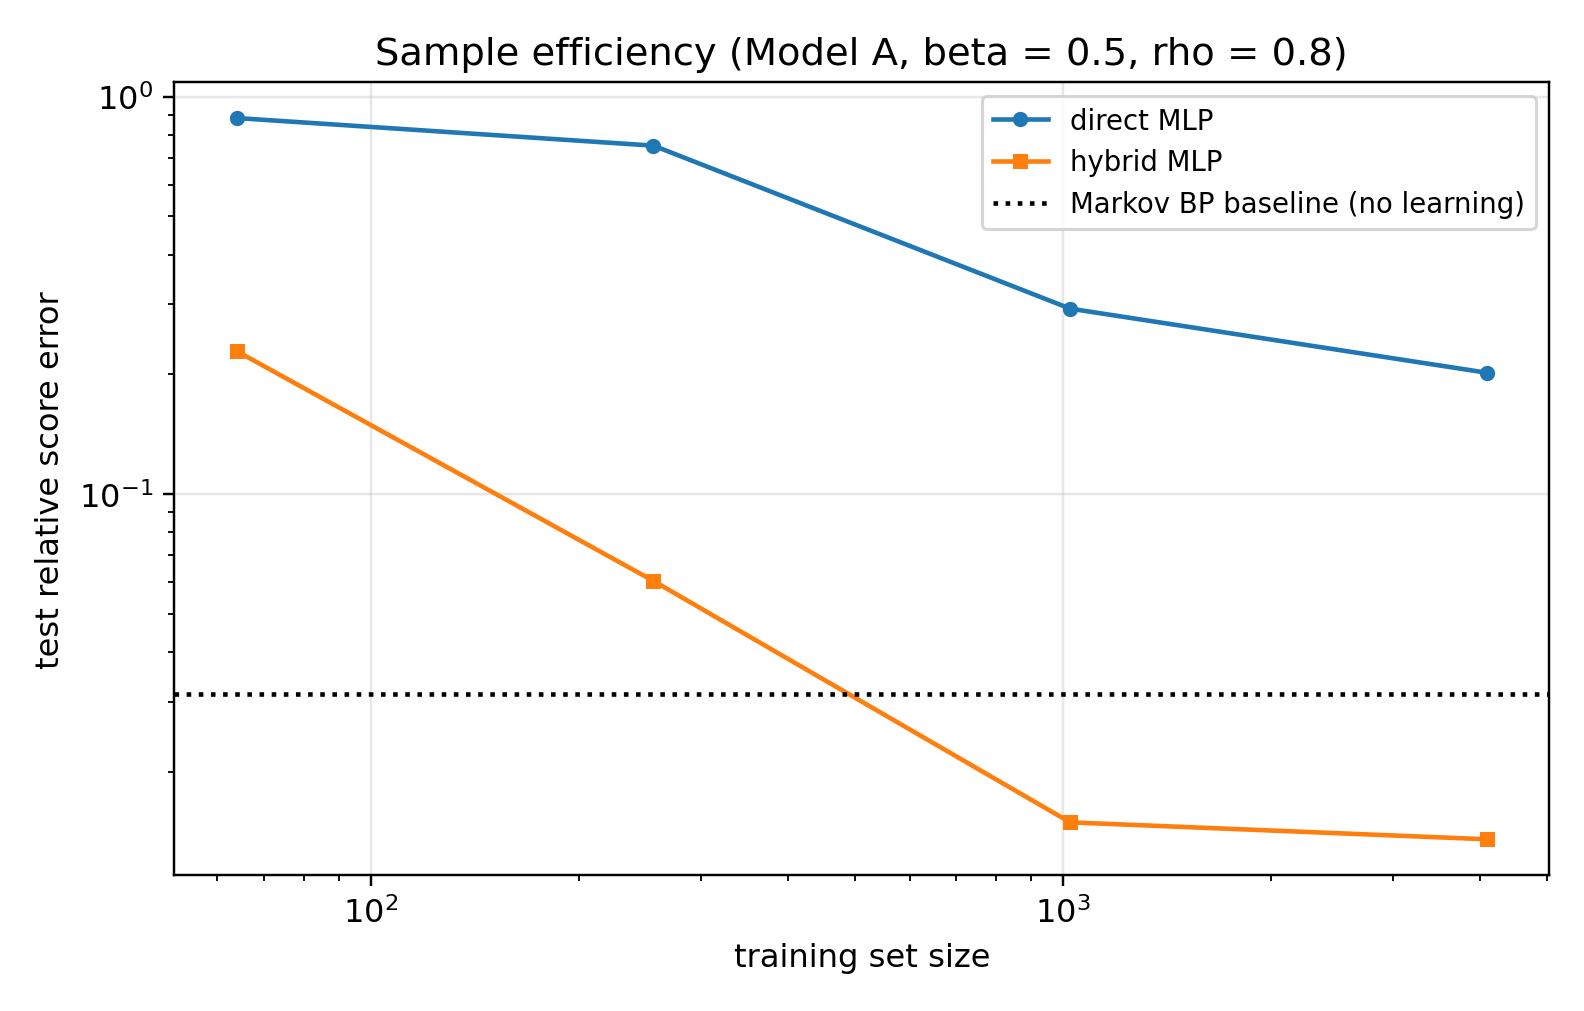
\includegraphics[width=0.49\textwidth]{../outputs/exp_04_approx_markovianity/hybrid_sample_efficiency.png}
  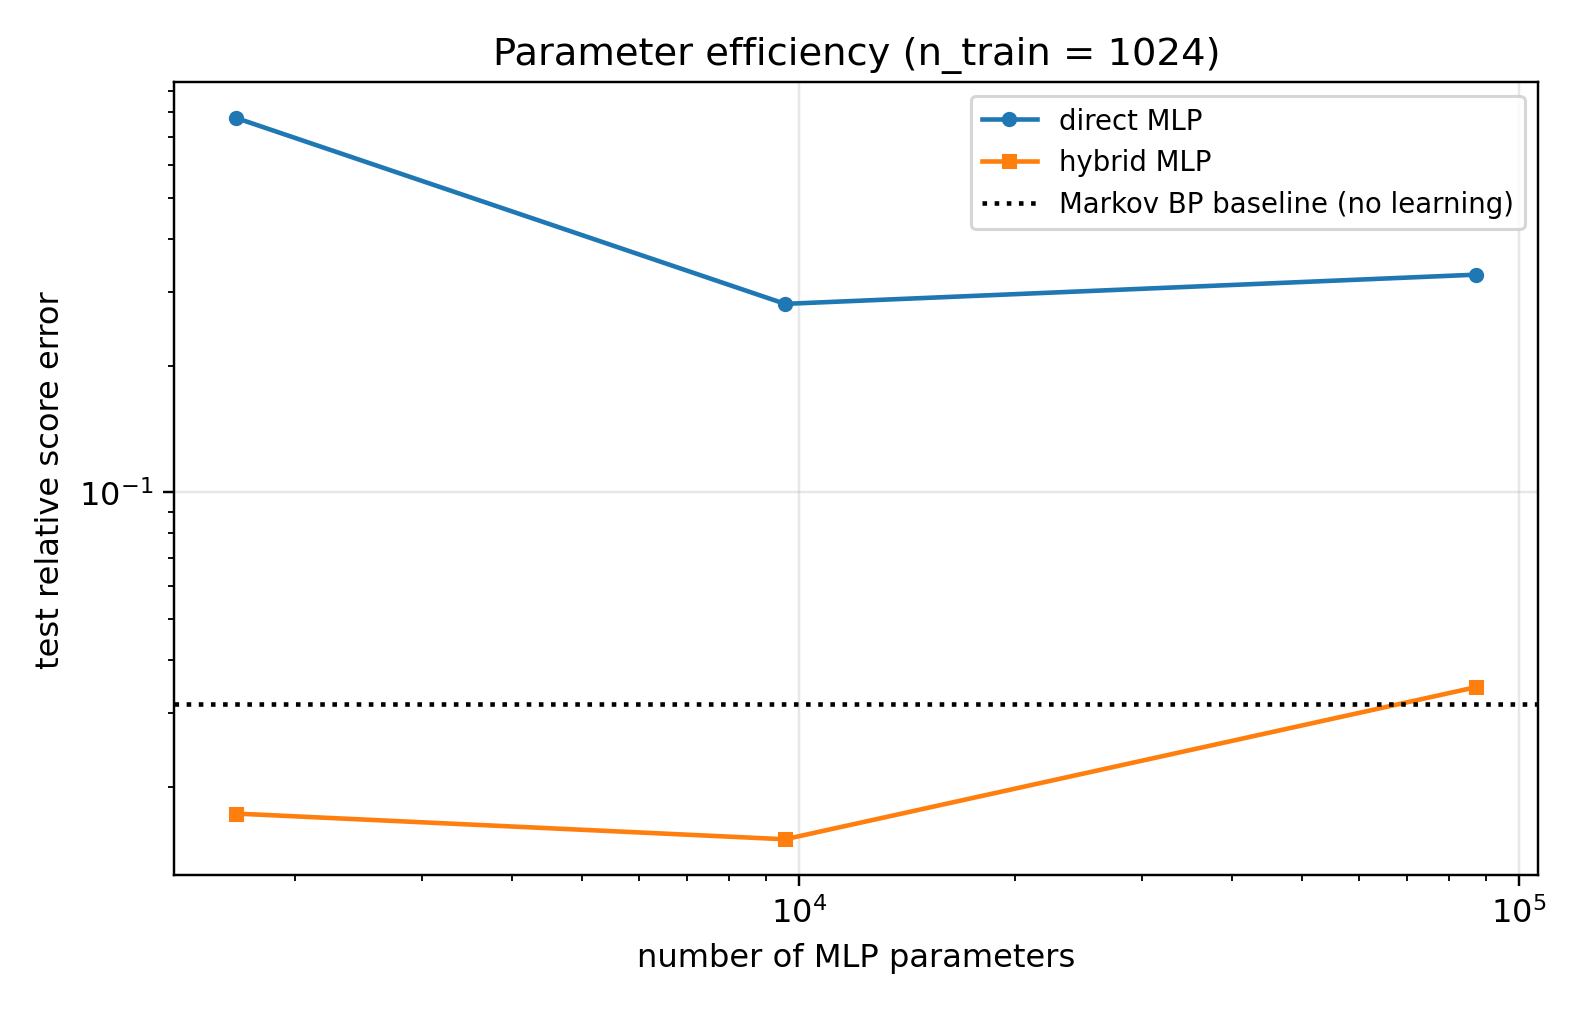
\includegraphics[width=0.49\textwidth]{../outputs/exp_04_approx_markovianity/hybrid_parameter_efficiency.png}
  \caption{Sample (left) and parameter (right) efficiency of direct vs hybrid score
  learning on Model A.}
  \label{fig:hybrid}
\end{figure}

\begin{remark}[Honest caveats]
The Markov model is \emph{known} here, not estimated ($K_\varphi$ given, not learned);
the comparison isolates the value of the structural baseline, not of a full estimation
pipeline. Targets are exact scores (supervised), not denoising score matching; the
sample-efficiency gap could change under DSM noise. And Model A is the friendly case:
its residual is exactly rank one and $x$-linear --- which is precisely the point: when
approximate Markovianity holds with low-rank corrections, the residual is a
\emph{much} easier learning problem than the full score.
\end{remark}

%=====================================================================
\section{Reverse-diffusion dynamics (exp.\ 05)}

Convention: reverse SDE
$x\leftarrow x + h\,(x+2s(x,t)) + \sqrt{2h}\,\xi$ integrated on a geometric grid from
$T=3$ to $t_{\min}=0.01$ (80 steps, 200 trajectories); probability-flow ODE
$\dot x = -x - s$ with Heun steps for reconstruction. Paired comparisons share initial
noise and Brownian increments.

\subsection{Does the Gaussian score wash out non-Gaussian structure?}

Generating from the Laplace chain ($\rho=0.85$) with the grid-BP score versus the
Gaussian-BP score:

\begin{center}
\begin{tabular}{lrrr}
\toprule
 & innovation exc.\ kurtosis & marginal var & lag-1 corr.\\
\midrule
clean prior samples & 2.72 & 0.94 & 0.837\\
reverse, grid-BP score & \textbf{2.86} & 1.06 & 0.828\\
reverse, Gaussian-BP score & \textbf{0.12} & 1.05 & 0.832\\
\bottomrule
\end{tabular}
\end{center}

Both samplers reproduce the second-order statistics; only the grid-BP score recovers
the heavy-tailed innovations. This is the dynamical face of Proposition
\ref{prop:equivalence}: the Gaussian score \emph{is} the score of a Gaussian model, so
its reverse diffusion generates (asymptotically) Gaussian samples --- the
non-Gaussianity is not distorted but \emph{erased}.

\begin{figure}[H]
  \centering
  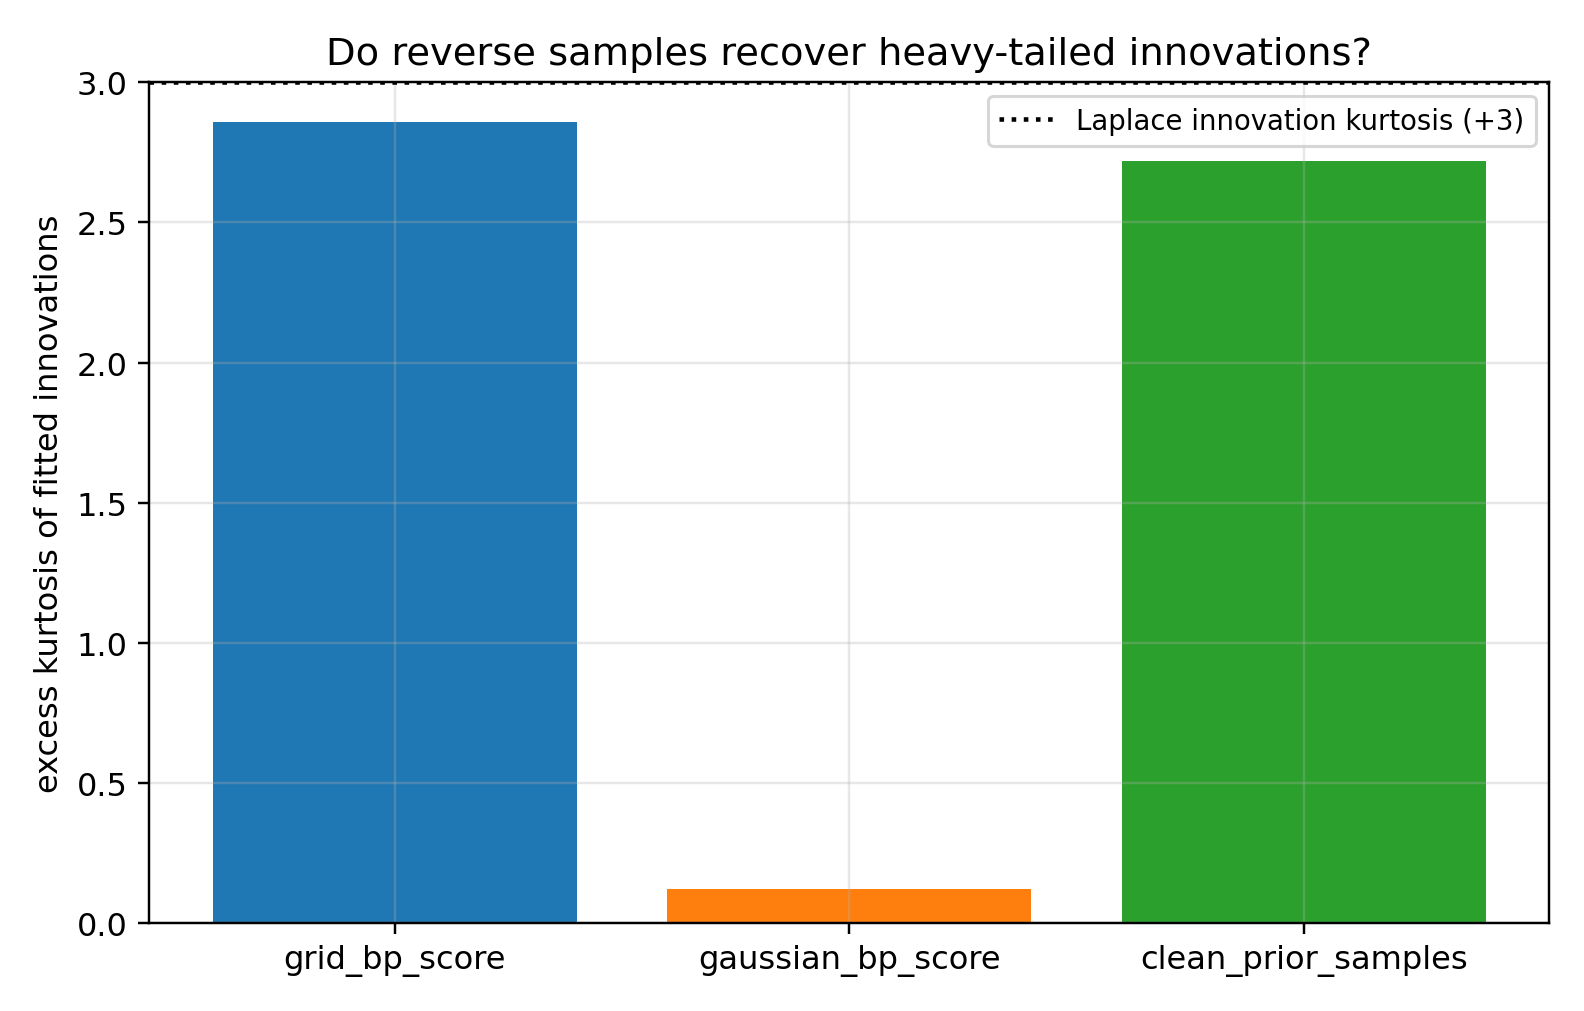
\includegraphics[width=0.49\textwidth]{../outputs/exp_05_reverse_dynamics/setup1_innovation_kurtosis.png}
  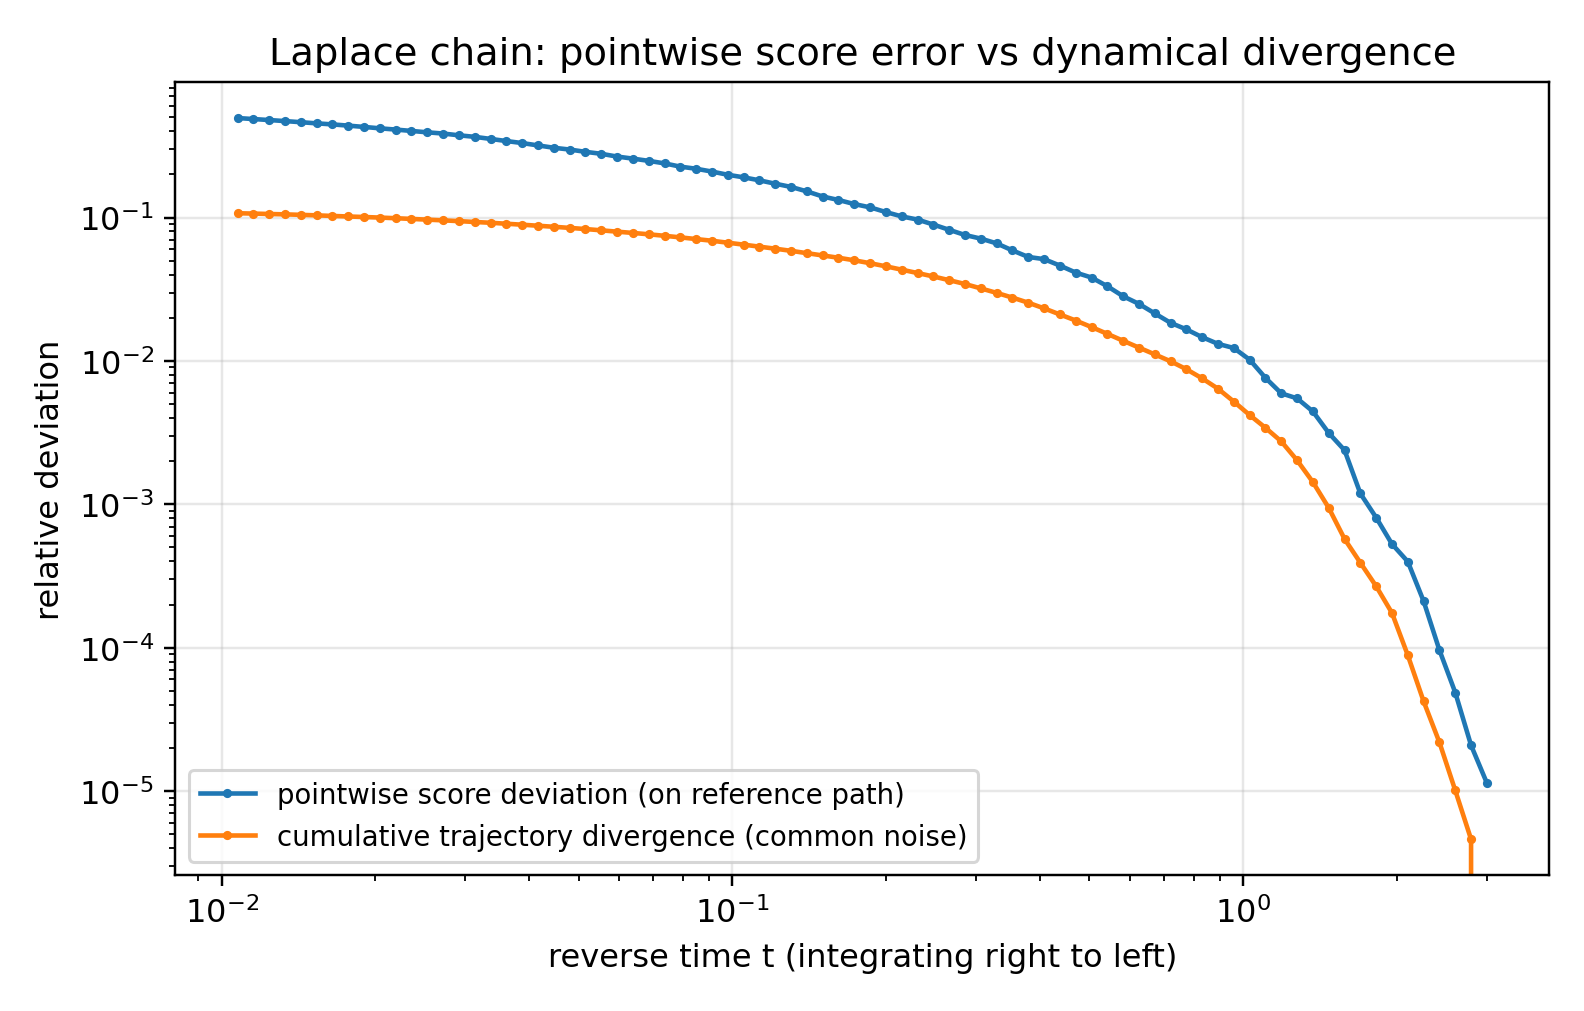
\includegraphics[width=0.49\textwidth]{../outputs/exp_05_reverse_dynamics/setup1_pointwise_vs_dynamic.png}
  \caption{Left: innovation kurtosis of reverse samples. Right: pointwise score
  deviation on the reference path vs cumulative common-noise trajectory divergence.}
  \label{fig:dyn}
\end{figure}

\subsection{Pointwise error vs dynamical error}

Along the reverse trajectory, the pointwise Gaussian-vs-grid score deviation is
$\sim10^{-5}$ at $t=3$, crosses $10^{-1}$ near $t\approx0.15$, and reaches $0.49$ at
$t_{\min}$; yet the cumulative trajectory divergence under common noise saturates
around $0.11$. Two conclusions. First, the dynamics are \emph{stable}: score error is
not amplified along the flow (the late-time contraction of the reverse SDE limits
accumulation; errors arrive mostly after the trajectory's large-scale structure is
frozen). Second, stability in $L^2$ is deceptive: the modest terminal displacement is
exactly what carries the higher-moment structure, as the kurtosis table shows. Small
pointwise score error at moderate $t$, plus stability, is \emph{not} sufficient for
distributional correctness in the tails.

Reconstruction from $t=1$ (probability-flow ODE) shows the two scores recovering
correlation with the clean sample nearly identically (second-order task, consistent
with the above); see \texttt{setup2\_correlation\_recovery.png}.

\subsection{Model A: recovering the global mode}

Generating from Model A ($\beta=0.5$) with four scores: exact, Chow--Liu Markov,
naive Markov, and hybrid (chain $+$ rank-one). Top eigenvalue of the terminal sample
covariance (true value $12.7$; finite-batch/discretization biases affect all samplers
equally --- exact-score value $10.5$):
exact $10.5$, hybrid $10.5$ (bitwise-identical trajectories, as
\eqref{eq:rank-one} is exact), Chow--Liu $8.1$, naive $5.6$. A Markov score cannot
generate the global collective mode; the rank-one correction restores it exactly.

\begin{figure}[H]
  \centering
  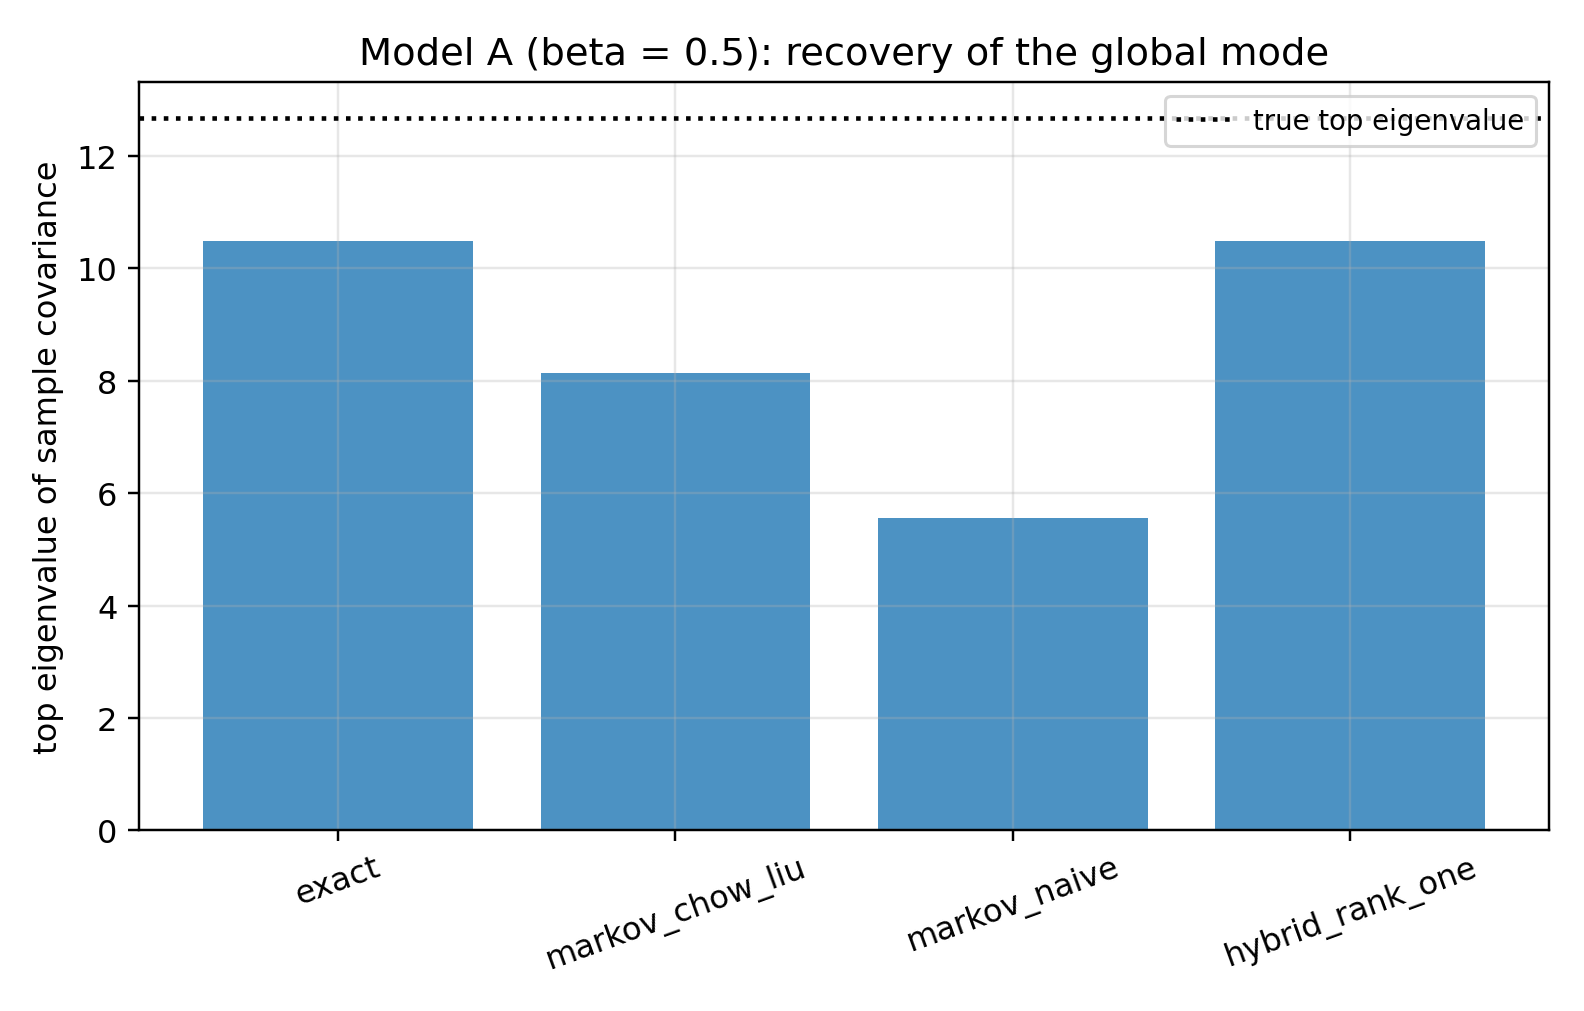
\includegraphics[width=0.6\textwidth]{../outputs/exp_05_reverse_dynamics/setup3_global_mode_recovery.png}
  \caption{Model A: top eigenvalue of the sample covariance of reverse-generated
  samples.}
  \label{fig:global-mode}
\end{figure}

%=====================================================================
\section{Interpretation, limitations, and next steps}

\paragraph{What is exactly established.}
(i) For Markov-chain priors under coordinatewise OU noising, BP computes the exact
score; the entire computational question is message representation.
(ii) Single-Gaussian projected BP on linear chains equals matched-Gaussian-model BP
(Prop.\ \ref{prop:equivalence}); its failure modes are therefore model failures:
erased tails and modes, worst at small $t$ by \eqref{eq:error-identity}.
(iii) For chain-plus-low-rank-latent Gaussian priors, the non-Markov score correction
is exactly low-rank (Prop.\ \ref{prop:woodbury}); augmented BP is closed-form.

\paragraph{What is numerically established.}
Grid BP is spectrally accurate and abruptly fails only below a predictable $t$;
with $M=401$, $A=8$ it is a sound reference for every experiment here. The corrected
Gaussian baseline degrades smoothly and predictably in $(t,\text{kurtosis},\rho)$.
Hybrid BP-plus-residual learning dominates direct score learning by an order of
magnitude on a model with genuine low-rank non-Markovianity. Reverse dynamics under
approximate scores are $L^2$-stable but distributionally wrong precisely in the
structure the approximation discards.

\paragraph{What this does not show.}
BP does not solve general diffusion models: real priors are unknown, non-chain, and
high-dimensional; our non-Gaussian ground truths are numerical (grid), not analytic;
the hybrid experiments assume the Markov model known and use supervised score targets.
Claims are limited to: \emph{if the clean distribution is (approximately) a Markov
chain, BP-based scores are exact (resp.\ structured baselines), and the non-Markov
residual can be dramatically simpler than the full score --- in the low-rank-latent
case, exactly rank one.}

\paragraph{Next steps, in order of leverage.}
\begin{enumerate}[leftmargin=1.6em]
  \item \textbf{Gaussian-mixture messages}: the first family where message error
  $\neq$ model error; measure how many components close the small-$t$ gap on the
  bimodal chains (the worst case found here).
  \item \textbf{Estimated $K_\varphi$}: learn the transition from data (parametric or
  nonparametric), quantify how transition-estimation error propagates through
  \eqref{eq:error-identity} to the score, completing the hybrid pipeline
  $s_{\rm BP,K_\varphi}+r_\theta$ end to end.
  \item \textbf{Denoising-score-matching training} of the residual (no exact targets),
  to test whether the sample-efficiency gap survives DSM variance.
  \item \textbf{Model C} (non-Gaussian chain $+$ global latent): Rao--Blackwellized
  BP with a quadrature over the latent times grid-BP chains --- machinery already in
  place; the reference is small-$n$ quadrature or particle methods.
  \item \textbf{Nonlinear transitions}, where Proposition \ref{prop:equivalence}
  fails and moment-matched messages genuinely differ from any Gaussian model ---
  the sharpest place to study message-level approximation per se.
\end{enumerate}

\appendix
\section{Package layout and reproduction}
\begin{center}
\begin{tabular}{ll}
\toprule
Path & Content\\
\midrule
\texttt{src/} & library: priors, noising, grid BP ($+$ evidence), information-form\\
 & Gaussian BP, exact scores, Markov approximations, numpy MLP, samplers\\
\texttt{experiments/exp\_01..05} & all experiments; \texttt{--quick} smoke mode; CSV/JSON/PNG outputs\\
\texttt{outputs/} & committed results of the full runs used in this report\\
\texttt{notebooks/01..04} & executed analysis notebooks\\
\texttt{tests/} & 14 pytest checks (exactness, identities, equivalence, convergence)\\
\texttt{audit/AUDIT\_NOTE.md} & full Layer-1 audit\\
\bottomrule
\end{tabular}
\end{center}
Determinism: all randomness flows through \texttt{src.utils.rng\_for} (seeded by
experiment/setting keys), so method comparisons are paired by construction. Provenance
(package versions, timestamps) is written into every \texttt{params.json}.

\section{Relation to the previous report}
The general theorem, its proof, and the Gaussian-closure algebra are unchanged from
\emph{From Gaussian AR(1) Belief Propagation to General Markov-Chain Diffusion Scores}
(July 2026) and are not repeated in full here. The Laplace-chain numbers of that
report remain valid at $t\le0.9$ and are superseded at $t\ge1.3$ by the corrected
baseline (artifact F1). Its interpretation of ``Gaussian message error'' should be
read as ``matched Gaussian model error'' per Proposition \ref{prop:equivalence}.

\begin{thebibliography}{9}
\bibitem{prevReport} G.\ Mantovani, \emph{From Gaussian AR(1) Belief Propagation to
General Markov-Chain Diffusion Scores}, internal project note, July 2026.
\bibitem{mezardMontanari} M.\ M\'ezard and A.\ Montanari, \emph{Information, Physics,
and Computation}, Oxford University Press, 2009.
\bibitem{anderson} B.\ D.\ O.\ Anderson, \emph{Reverse-time diffusion equation
models}, Stochastic Processes and their Applications, 1982.
\bibitem{minka} T.\ Minka, \emph{Expectation Propagation for approximate Bayesian
inference}, UAI 2001. (Assumed-density filtering and moment projection.)
\bibitem{biroliMezard} G.\ Biroli and M.\ M\'ezard, \emph{Generative diffusion in very
large dimensions}, arXiv:2306.03518, 2023.
\bibitem{dynamicalRegimes} G.\ Biroli, T.\ Bonnaire, V.\ de Bortoli, M.\ M\'ezard,
\emph{Dynamical Regimes of Diffusion Models}, arXiv:2402.18491, 2024.
\bibitem{unetBP} S.\ Mei, \emph{U-Nets as Belief Propagation}, arXiv:2404.18444, 2024.
\end{thebibliography}

\end{document}
